\documentclass[11pt]{report}

% the recommended packages discussed in section 4. Keep them!
\usepackage{pkgs/rtsched}
\usepackage[sorting=none]{biblatex}
\usepackage{parskip}
\usepackage{booktabs}
\usepackage{siunitx}
\sisetup{per-mode=symbol} 
\usepackage{pgfgantt}
\usepackage{rotating}
\usepackage{vhistory}
\usepackage{pgfplots}
% \usepgfplotslibrary{external}
% \tikzexternalize
\usepackage{pgfplotstable}
\usepackage{tikz}
\usepackage{caption}
\usepackage{subcaption}
\usepackage{adjustbox}
\usepackage{eqexpl}
\eqexplSetIntro{where:} % set parenthesis in the left of the first item
\eqexplSetDelim{=} % set delimiter to "="
\usepackage{bytefield}
\usepackage{xcolor}
\usepackage{amsfonts}
\usepackage{amsmath}
\usepackage{graphicx}
\usepackage{wheelchart}
\usepackage{etoolbox}
\usepackage{listofitems}
\usetikzlibrary{decorations.text}
\usepackage{lipsum}
\usepackage{import}
\usepackage[colorinlistoftodos]{todonotes}
\usepackage{pgf-pie}  
\usepackage{multirow}
\usepackage{threeparttable}

\definecolor{lightcyan}{rgb}{0.84,1,1}
\definecolor{lightgreen}{rgb}{0.64,1,0.71}
\definecolor{lightred}{rgb}{1,0.7,0.71}
\definecolor{lightorange}{rgb}{1,0.8,0.5}
\definecolor{lightpurple}{rgb}{0.89,0.79,0.96}
\definecolor{lightyellow}{rgb}{0.92,0.99,0.48}
\definecolor{lightgray}{gray}{0.8}

% \definecolor{blue}{rgb}{0,0,1}
\definecolor{bluehue1}{RGB}{0, 76, 109}
\definecolor{bluehue2}{RGB}{17, 109, 141}
\definecolor{bluehue3}{RGB}{38, 143, 173}
\definecolor{bluehue4}{RGB}{63, 180, 202}
\definecolor{bluehue5}{RGB}{92, 217, 230}
\definecolor{bluehue6}{RGB}{126, 255, 255}

% some packages required for typesetting a nice manual
\usepackage{tabularx}
\usepackage[a4paper]{geometry}
\usepackage{listings}
\lstset{language=tex, frame=single, basicstyle=\small}
\usepackage{shortvrb}
\MakeShortVerb{\|}
\usepackage{titlesec}
\newcommand{\sectionbreak}{\clearpage}

% load the titlepage providing package. Mind the slash!
\usepackage[affiliation=double,corporate-identity=none]{tu/e}

% its good practice to always load the ~ref packages last, in this order:
\usepackage{hyperref}
\hypersetup{colorlinks=true,urlcolor=blue,linkcolor=blue,citecolor=red}
\usepackage[nameinlink]{cleveref}

\DeclareMathOperator{\eread}{E_{\textrm{read}}}
\DeclareMathOperator{\ereadlpddr5x}{E_{\textrm{read,LPDDR5X}}}
\DeclareMathOperator{\ereadpcm}{E_{\textrm{read,PCM}}}
\DeclareMathOperator{\ephy}{E_{\textrm{phy}}}
\DeclareMathOperator{\ectrl}{E_{\textrm{ctrl}}}
\DeclareMathOperator{\eaxi}{E_{\textrm{axi}}}
\DeclareMathOperator{\enoc}{E_{\textrm{noc}}}
\DeclareMathOperator{\ewrite}{E_{\textrm{write}}}
\DeclareMathOperator{\econf}{E_{\textrm{conf}}}
\DeclareMathOperator{\econflpddr5x}{E_{\textrm{conf,LPDDR5X}}}
\DeclareMathOperator{\econfpcm}{E_{\textrm{conf,PCM}}}
\DeclareMathOperator{\eproc}{E_{\textrm{proc}}}


% Use these macros to supply information for on your titlepage. The must be
% placed in the preamble! You can safely omit any of them if you don't want to
% print that specific bit of information to the titlepage.
\title{Exploring efficient reconfiguration on the GrAICore}
% \subtitle{Hello world}
\thesistype{Master thesis}
\idnumber{1712918}
\author{S. Yip}
\supervisors{Supervisors\\dr.ir. M.C.W. Geilen (TU/e)\\dr. Hamid Tabani (Snap Inc.)\\dr.ir. Orlando Moreira (Snap Inc.)}
\version{Draft version}
\citydate{Eindhoven, November 2024}
\institutioninfo{Department of Electrical Engineering\\Electronic Systems Group}
\secondinstitutionlogo[height=2cm]{assets/snap_logo.png}
\secondinstitutioninfo{Snap Inc.\\Snap Lab Hardware Engineering}

\addbibresource{references.bib}

% \linespread{1.5}
\begin{document}
\onehalfspacing

\begin{versionhistory}
  \vhEntry{0.1}{September 30, 2024}{S. Yip}{Initial draft}
  \vhEntry{0.2}{October 22, 2024}{S. Yip}{Second draft}
\end{versionhistory}
Modern computer vision applications rely heavily on complex neural networks, often exceeding the memory capacity of resource-constrained processors found in edge devices.

This thesis investigates the use of off-chip memory to enable such processors---in particular the \graicore{}---to execute large and multiple computer vision models efficiently.

The challenge lies in the inherent limitations of the \graicore{}.
Its design requires the \graicore{} to have an AI model loaded locally before it can be utilized for inference.
Furthermore, the presence of limited on-chip memory and external interface limits the ability to load large models and transfer data rapidly.
In this context, large models are models that do not fit on the \graicore{} due to their size exceeding the on-chip memory capacity.
Executing multiple models means that two or more models are used by the \graicore{} while it is online.
These models are assumed to fit on the \graicore{}, but not at the same time.

Execution of these models is done by high-speed reprogramming or reconfiguration of the \graicore{} by transferring the relevant model data to its on-chip memory.
Specifically, we explore the architectural adaptations required to facilitate high bandwidth data transfers to the \graicore{} while maintaining sustainable power consumption.

Part of this study is the investigation into how breaking down large models into smaller parts (partitioning) makes them more manageable for processing by the \graicore{}.
It was found that an optimal partitioning strategy for large models for execution on the \graicore{} is a complex problem when targeting high performance.

Furthermore, LPDDR5X and PCM are explored as potential external memory technology solutions, examining the end-to-end energy consumption when performing model reconfiguration.
Findings demonstrate that on average around 23\% and 12\% is consumed by reconfiguration and the rest for the processing part for LPDDR5X and PCM respectively.
The ratio for reconfiguration can be further reduced by avoiding the transfer of certain redundant data.

This research contributes to the development of a more feature-rich and future-proof \graicore{}, enabling it to efficiently execute large and multiple models during runtime.


\tableofcontents

\chapter{Introduction}
\import{sections/introduction}{problem_statement}
\import{sections/introduction}{research_question}
\import{sections/introduction}{outline}

\chapter{Background}
\import{sections/background}{edge_ai}
\import{sections/background}{computer_vision}
\import{sections/background}{neural_networks}
\import{sections/background}{ai_accelerator}
\import{sections/background}{noc}
\import{sections/background}{external_memory}
\import{sections/background}{graicore}
% \import{sections/background}{swapping}

\chapter{Evaluation of the config NoC}
\import{sections}{config_noc_eval}

\chapter{Model execution analysis}
\import{sections/model_execution_analysis}{multi_model}
\import{sections/model_execution_analysis}{large_model}

\chapter{Config NoC bandwidth improvements}
\import{sections/bandwidth_improvements}{bandwidth_improvements}
\import{sections/bandwidth_improvements}{proposed_changes}

\chapter{Power analysis} \label{chapter:power_analysis}
\import{sections}{power_analysis}

\chapter{Model configuration improvements} \label{chapter:model_configuration_improvements}
\import{sections}{model_configuration_improvements}
\import{sections/model_configuration_improvements}{states}
\import{sections/model_configuration_improvements}{weight_duplications}
\import{sections/model_configuration_improvements}{pruning}
% \import{sections/model_configuration_improvements}{quantization}
\import{sections/model_configuration_improvements}{conclusion}

% \chapter{Exploring partitioning strategies}

\chapter{Partitioning large models - Formal problem description}
% \section{Large model partitioning}
\label{section:tmp}
\lipsum[1]

\chapter{Conclusion}
\lipsum[1]

\chapter{Future work}
\section{Exploring partitioning strategies}
\import{sections}{exploring_partitioning}
\section{Parallel configuration/processing}
Explain that we can speed up inference of large models by configuring and processing the partitions in parallel or pipelined.

\section{Compiler analysis}
Explain that with a comprehensive analysis of the compiler, we can improve the search for optimal solutions for a model or model partition.

\section{Add static power consumption}
Explain that we have only considered dynamic power/energy consumption.
Static power has not been explored.

\section{Other memory technologies}
We have only explored two specific memory technologies (DDR).
Using an other memory technology may provide us with better results.
This could be in terms of speed and energy use.

The energy numbers of PCM looks more promising compared to the LPDDR5X memory.
However, a few parameters haven't been considered in this research.
For example, the density (capcity per physical area) of LPDDR5X is higher than PCM.

\section{}
% Recent trends in artificial intelligence (AI) development indicate a substantial surge in the complexity and size of AI models since the advent of the Deep Learning Era \cite{EpochDatabaseVisualization}.
Sophisticated state-of-the-art AI models, such as those used in natural language processing and image recognition, can vary widely in complexity, with some containing as few as thousands of parameters and others exceeding a trillion.
These parameters are the fundamental components that AI models manipulate to learn from data and make predictions or decisions.
Processing such huge models requires an extensive amount of computational power.
High-performance computing systems with powerful GPUs and large memory pools are typically employed to train these models as well as to perform inference using them.
However, the deployment of AI solutions is not limited to these high-resource environments.
There is a significant push to bring AI capabilities closer to the end-users, which is where edge computing comes into play.
This shift is primarily motivated by the need for reduced latency, ensuring that decisions and actions can be taken almost instantaneously, and by the importance of low power consumption.



% \section{Problem statement}

The problem to be addressed by this project is the inability to reconfigure the GrAICore during run-time.
The current design of the GrAICore is incapable of doing this due to the limited host to GrAICore interface.
Adding this feature for the GrAICore to reconfigure during run-time significantly enhances its capabilities.
Firstly, it will allow multiple computer vision models to be used simultaneously while the GrAICore is running.
Deploying multiple computer vision models can be highly beneficial for creating a multifaceted system capable of handling diverse tasks simultaneously.
Each model can be specialized for a specific function, allowing the system to be more versatile and responsive to different visual processing requirements.
Secondly, using a technique such as partitioning the neural network into parts, allows the GrAICore to manage large models that do not fit on the GrAICore at once.
This method processes one model part at a time, requiring only a part of the model to be loaded.
Larger computer vision models for inference typically offer higher accuracy and better generalization to new data, can capture more complex features, and are more robust to noise and distortions.
They are valuable for tasks requiring the utmost precision.

Additionally, as specified by GML, they require that the GrAICore supports seamless reconfiguration.
In this context, seamless reconfiguration refers to the ability to switch between different AI models, or to modify the current model, without interrupting or significantly delaying data processing.
Given that the GrAICore is focused on computer vision applications, this means that it is crucial that the processing of input images occurs in a timely manner.
This is particularly challenging for video applications, where each frame must be processed before the next one arrives. Failing to meet this requirement can reduce the usefulness of the results, thereby degrading the system's quality of service.
Specifically, GML requires the system to support an incoming video frame rate of \SI{60}{FPS}.

% \section{Research question}

Due to the limited local memory of the \graicore{}, it can only support AI models of a certain size.
This limitation becomes a roadblock for scenarios where larger models are needed for improved accuracy or when multiple models need to be deployed simultaneously.
The introduction of external memory is a potential solution to this challenge, but it requires careful integration to maintain the energy efficient, high-speed and low-latency performance expected from edge devices.

Ultimately, this project aims to answer the following research question:

\textbf{How can the architectural design of the \graicore{} be adapted to enable seamless reconfiguration?}

To address this overarching question, the project will explore several sub-research questions:

\begin{itemize}
    \item \textbf{Supporting multiple models:}
    \begin{itemize}
        \item What modifications are necessary to support switching between multiple AI models for videos up to \SI{60}{FPS}?
    \end{itemize}
    \item \textbf{Supporting large models:}
    \begin{itemize}
        \item What strategies can be employed to support the execution of large AI models?
    \end{itemize}
    \item \textbf{Sustainable power consumption:}
    \begin{itemize}
        \item How can sustainable power consumption be ensured while maintaining performance?
    \end{itemize}
\end{itemize}
% \section{Outline}

\lipsum[1]


% \chapter{Background}

\lipsum[1]

% \subsection{AI at the edge}
% \input{sections/background/edge_ai}

% \subsection{GrAICore}
% \section{\graicore{}}
In this research, we focus on the \graicore{}, a many-core AI accelerator designed specifically for edge devices.
The \graicore{} utilizes the ``NeuronFlow'' technology that is inspired by the neural structures of the brain \cite{moreiraNeuronFlowNeuromorphicProcessor2020}.
The \graicore{} prioritizes energy efficiency while offering specialized hardware for execution of neural networks. 
Its main use case is computer vision applications using models based on convolutional neural networks (CNNs).
It features a total of 144 neuron cores, arranged in a 12 by 12 grid.
% A neuron core includes a local SRAM memory for storing data such as model parameters and a processing element for performing mathematical operations (see \cref{fig:neuron_core}).

% \begin{figure}[htbp]
%     \centering
%     \includegraphics[width=0.4\textwidth]{assets/neuron_core.pdf}
%     \caption{The neuron core includes a processing element (core) and a local memory (a.k.a. unified memory)}
%     \label{fig:neuron_core}
% \end{figure}

Each neuron core is connected to a distinct SRAM, which stores all the relevant information for processing incoming events.
A neuron core uses an event processing pipeline to handle incoming events from an input sensor or other neuron cores.
These events include the input data or activation data of the previous stage.
For each event received, relevant information is retrieved from the SRAM (such as weights) to instruct the arithmetic logic unit (ALU) to perform the necessary logical operations.
Each event can result in the update of multiple neuron states inside its SRAM.
A new event is generated if a particular activation value is non-zero.
This new event is then sent to the next neuron core for further processing.

\subsection{Mapping}
Before an AI model can be used on the \graicore{}, the model must first be mapped for the \graicore{} and configured on the \graicore{}.
Mapping models or neural networks on the \graicore{} demands a strategic approach to distributing the computational workload.
This involves carefully segmenting the network, which can be done at the layer level, neuron level, or a combination of both, depending on the network's structure. 
A key objective is to balance the computational load across the neuron cores while minimizing communication overhead and maximizing the use of on-chip memory.
Efficient dataflow management is also critical.
This can involve employing data parallelism, where different neuron cores process different batches of data, or model parallelism, where different parts of the model are distributed across neuron cores.
Pipelining can further enhance efficiency by dividing the computation into stages and allowing concurrent execution.
Communication between neuron cores is another crucial factor.
The \graicore{} employs specialized interconnect networks to facilitate efficient data exchange.
% Synchronization mechanisms ensure correct execution, and collective operations are used to aggregate results from multiple cores.
While this mapping process can be complex, a specialized compiler has been made to automate these tasks.
This compiler analyzes the neural network and generates optimized code that efficiently utilizes the \graicore{}'s available resources.

\subsection{Near-memory computing}
The \graicore{} makes use of near-memory computing.
Near-memory computing refers to a computer architecture where computation is performed close to the memory.
This approach aims to mitigate the ``von Neumann bottleneck'', a limitation caused by the traditional computing architecture where the CPU (Central Processing Unit) and memory are separate entities, and data must be transferred back and forth between them \cite{indiveriMemoryInformationProcessing2015}.
By performing computations closer to where data is stored, data movement between the processing element and memory is minimized, reducing latency and energy consumption.
However, this introduces a constraint that requires the parameters of a model to reside in local memory before it can be used by the processing element.
Thus, an AI model must first be mapped and loaded onto the \graicore{} before it can be used for inference.
% Mapping means to assign the layers of a neural network to the neuron cores.
% Intelligent mapping is important for balancing memory, computation and traffic between neuron cores.
The \graicore{} features a total of \SI{36}{MB} of local memory, which is evenly distributed across its $144$ neuron cores.

The size of an AI model can be quantified by the number of its parameters.
For instance, if a parameter is stored as a 16-bit value on the \graicore{}, it can accommodate approximately $\frac{\SI{36}{MiB}}{\SI{16}{b}}$ parameters\footnote{In practice, the available space for parameters is smaller because a portion of the memory is allocated for storing other relevant data.}, which translates to around \SI{19}{M} parameters in total.
Popular computer vision models like ResNet-50 \cite{heDeepResidualLearning2015} and YOLOv7 \cite{wangYOLOv7TrainableBagoffreebies2022}, with over \SI{25}{M} and \SI{37}{M} parameters respectively, are already too large by themselves to fit on the \graicore{}.
Using optimization techniques, these models can be compressed into a smaller size.
For example, YOLOv7-tiny \cite{wangYOLOv7TrainableBagoffreebies2022} is a size optimized model of the YOLOv7 for edge devices at the cost of accuracy.
Its size is decreased to around \SI{6}{M} parameters, making it suitable for the \graicore{}.
Furthermore, it has been demonstrated that the ResNet-50 model can be mapped on the \graicore{} after pruning around 80\% of the parameters and quantizing the remaining parameters to 8 bits.
% In summary, the number of parameters that can be stored on the \graicore{} is limited by the size of its on-chip memory.

% TODO change to subcaption
\begin{figure}[htbp]
    \centering
    \subfloat[The \eventnoc{} features a 2D torus topology]{
        \includegraphics[width=0.45\textwidth]{assets/event_noc.pdf}
        \label{fig:event_noc}
    }
    \hfill
    \subfloat[The \confignoc{} features a 2D mesh topology]{
        \includegraphics[width=0.45\textwidth]{assets/config_noc.pdf}
        \label{fig:config_noc}
    }
    \caption{\graicore{}'s network-on-chips. A neuron core (NC) communicates via its associated router (R) with other neuron cores and external parties such as the host device (not illustrated).}
    \label{fig:noc}
\end{figure}

\subsection{NoCs}
The neuron cores are connected to each other with two distinct network-on-chips (NoCs), each serving its own purpose (see \cref{fig:noc}).
Firstly, the \eventnoc{} is used for exchanging activated neuron states in the form of small messages called Events.
Events are only generated when an AI model is being executed.
The \eventnoc{} uses the 2D torus topology.
Secondly, the \confignoc{} is responsible for configuring the \graicore{}, monitoring and debugging.
The \confignoc{} uses a different topology, namely a 2D mesh topology.
Configuring the \graicore{} means that the local memories of the neuron cores are written with the parameters of an AI model.
A host device (e.g., a microcontroller) initiates the configuration of the \graicore{}.
The host device is connected to the \confignoc{} via a single link, which is used to transfer data to and from any neuron core.
Since all data transfers must go through this link to reach its destination neuron core, it causes a significant bottleneck in data transfer speed to the \graicore{}.
That is, the amount of data that can be transferred to the neuron cores within a certain time is poor as it was not designed with speed in mind.
Therefore, currently, the configuration of the memories of the neuron cores is only performed once at the start.
% This limitation restricts the \graicore{} to be (partially) reconfigured at run-time.



% \subsection{Network-on-chip}
% \section{Network-on-chip}
Network-on-chip (NoC) has become a crucial component for data communication in modern processors, offering high throughput, low latency, and efficient power utilization.
The performance of NoCs is influenced by various factors such as topology, routing algorithms, switching mechanisms, and link/channel width.
With the goal in achieving optimal performance, researchers have looked into exploring different aspects of NoC design to enhance its efficiency.
One key element that significantly impacts NoC performance is the choice of topology.
Studies have shown that selecting an appropriate topology is critical as it affects zero-load latency, sustainable bandwidth, and power consumption \cite{chenPhysicalVsVirtual2010}.
For instance, the 2D mesh topology (see \cref{fig:config_noc}) is commonly used in NoCs due to its scalability and ability to support efficient communication among cores.
This topology allows for straightforward routing and is well-suited for large-scale systems \cite{sanchezAnalysisOnchipInterconnection2010}. 

Routing algorithms play a crucial role in determining the efficiency of data transmission in NoCs.
Research has focused on developing novel routing algorithms to optimize performance.
For example, a study introduced a low-latency routing algorithm that exploits path diversity to achieve high bandwidth and low latency in NoC routers \cite{yangExploitingPathDiversity2012}.
Furthermore, the design of energy-efficient routing algorithms has been explored to enhance the overall power efficiency of NoCs \cite{parikhPowerAwareNoCsRouting2014}.
These routing algorithms aim to balance the trade-off between performance metrics such as throughput and latency while minimizing power consumption.
The current configuration procedure for the \graicore{} transmits data packets from an external source to the destination neuron cores in a sequential manner, utilizing the XY routing algorithm \cite{glassTurnModelAdaptive1992}.
XY routing, being a non-adaptive algorithm, ensures that data packets always traverses the same path from source to destination.
Consequently, the traffic pattern remains straightforward.
At a time, there is only a single flow of data from source to destination.
Because of this, no parallel communication occurs during the configuration process and therefore the congestion is minimal.
However, if we choose to explore a NoC design or configuration procedure that involves concurrent traffic through the network, potential congestion issues may arise.
In such cases, a suitable routing algorithm must be implemented to manage and mitigate congestion effectively.

Switching techniques in NoCs determine how data packets are forwarded within the network, thereby influencing bandwidth, latency and power consumption.
Research has proposed energy-efficient reconfigurable circuit-switched NoCs as a means to optimize power utilization while maintaining high performance \cite{wolkotteEnergyEfficientReconfigurableCircuitSwitched2005}.
Additionally, studies on switching techniques with reduced buffer requirements highlight the importance of balancing performance and power efficiency in modern NoC designs \cite{requenaEfficientSwitchingTechnique2008}.
By implementing efficient switching mechanisms, designers can achieve lower power consumption without compromising network performance.

Link width is another essential design parameter that influences the overall bandwidth of the network.
Wider links can accommodate higher data rates, leading to improved throughput and reduced latency.
However, the use of wider links also consumes more power, so there is a trade-off between performance and power consumption that designers need to consider when designing a NoC \cite{manhokimNetworkonchipLinkAnalysis2006}.
Widening the link widths in the \graicore{}'s NoC is a relatively straightforward enhancement, making it an appealing solution for improving both throughput and latency.
However, it is important to note that increasing the link widths also requires more silicon area due to the need for additional physical wires and increased router complexity.


% \subsection{External memory}
% \section{External memory}

Selecting the appropriate memory technology is critical for optimizing performance and energy efficiency.
For example, DRAM (Dynamic Random Access Memory) and NVM (Non-Volatile Memory) each present unique advantages: DRAM is known for its high speed and throughput, making it suitable for performance-intensive tasks, while NVM offers non-volatility and energy efficiency, ideal for data persistence and energy-conscious applications.
Advanced techniques such as burst transfers and parallel data interfaces can further enhance memory system performance.
Additionally, optimizing both the memory controller and Network-on-Chip (NoC) for energy efficiency is essential to achieve balanced, high-performing many-core architectures.

DRAM technology is a prevalent choice for main memory in many-core systems due to its high density and cost-effectiveness \cite{oExploringEnergyefficientDRAM2011}. Furthermore, DRAM offers fast access times and high throughput, making it suitable for applications necessitating real-time data processing. Its ability to rapidly read and refresh data contributes to its widespread adoption in performance-critical environments.
Conversely, NVM technologies provide non-volatility, high capacity, and energy efficiency, making them ideal for storing large data volumes in edge devices. NVM technologies, such as Flash memory and emerging solutions like Phase-Change Memory (PCM), present a compelling alternative to traditional volatile memory.
While DRAM excels in performance, NVM technologies are increasingly competitive and offer a compelling alternative, particularly in scenarios prioritizing energy efficiency and data persistence \cite{dulloorSystemSoftwarePersistent2014}.

PCM (Phase-Change Memory) is a notable NVM technology that leverages the unique properties of chalcogenide glass to store data \cite{meenaOverviewEmergingNonvolatile2014}.
PCM operates by changing the state of the material between amorphous and crystalline phases, which correspond to different resistance levels representing binary data.
One of the significant advantages of PCM is its superior read performance compared to traditional Flash memory.
PCM can achieve read latencies comparable to DRAM \cite{wangExploringHybridMemory2013}, making it suitable for read-intensive applications where quick data retrieval is critical.
Moreover, PCM's endurance and reliability are notable.
Unlike DRAM, which requires periodic refreshing to maintain data integrity, PCM retains data without power, significantly reducing energy consumption in standby modes.

Burst transfers play a crucial role in improving the performance of external memory systems.
By allowing for the transfer of a block of data in a single contiguous sequence, burst transfers reduce the overhead associated with individual data transfers, thereby enhancing throughput \cite{bakhodaDesigningOnchipNetworks2013}.

To further enhance performance, utilizing multiple external memory interfaces for parallel data transfers can improve overall throughput.
By enabling simultaneous data transfers through different interfaces, the system can leverage parallelism to maximize memory bandwidth utilization, particularly beneficial in many-core architectures with multiple cores accessing external memory concurrently \cite{chenIncreasingOffchipBandwidth2014}.

In the context of energy consumption, both external memory and the NoC contribute significantly to the overall power consumption of the system.
The memory controller, which manages data transfers between the processor and external memory, consumes a considerable amount of energy \cite{udipiRethinkingDRAMDesign2010}.
Additionally, the NoC, which facilitates communication between cores in a many-core chip, may also consumes a substantial portion of the system's energy budget \cite{ziaHighlyscalable3DCLOS2010}.
Optimizing the design of the memory controller and the NoC for energy efficiency is crucial for enhancing the overall energy performance of many-core systems.

When considering the integration of external memory with a NoC in a many-core chip, it is essential to address performance metrics such as throughput, latency, and energy consumption.
The choice between DRAM and NVM technologies for external memory impacts these metrics significantly, with NVM technologies offering potential advantages in terms of energy efficiency.
Burst transfers and parallel data transfer interfaces are key mechanisms for improving throughput in external memory systems, while optimizing the energy consumption of the memory controller and the NoC is vital for enhancing the overall energy efficiency of many-core systems at the edge.


% \subsection{Swapping}
% \section{Swapping}

A technique that is similar to our plan of action is called swapping.
Swapping involves dynamically loading and unloading part of the model or data into and out of the device’s memory during inference or execution time \cite{wangSwapNetEfficientSwapping2024, huangSwapAdvisorPushingDeep2020}.
\cite{wang_swapnet_2024, huang_swapadvisor_2020}
When a large model cannot fit in the device’s memory. Parts of the model (e.g., layers) are stored in slower, but larger storage.
These parts are then loaded into the device’s memory on-demand during execution.
The device is responsible for scheduling the execution of the model parts so that the necessary chunks are loaded into the device’s memory in time for computation.
This will require careful timing to ensure that data is ready when needed to avoid stalling the processor.
Swapping introduces latency, as loading data from the slower storage takes time.
It is therefore crucial that this overhead is minimized to ensure that performance is acceptable.

Research has been done on using the swapping technique for supporting large neural networks on tiny microcontrollers in \cite{miaoEnablingLargeNeural2021}.
This is achieved by dynamically swapping neural network parts between a microcontroller's tiny SRAM and its large, low-cost external flash.
Although they managed to address the challenge of running large models on a resource-constrained edge device without accuracy loss, a microcontroller's hardware architecture is significantly different compared to that of the GrAICore's.
With low-cost microcontrollers as their target, the external flash bandwidth is usually poor ($<\SI{100}{MB/s}$).
As a consequence, the throughput of processed frames per second is also poor.
But despite that, the proposed scheduling technique shows promising results for executing large models on microcontrollers and can potentially be extended to be used on the GrAICore.
% \input{sections/background/edge_ai}
% \section{Computer vision}

Computer vision (CV) is a field of artificial intelligence (AI) that enables machines the ability to interpret, analyze and understand visual data from images and videos.
CV seeks to replicate the visual capabilities of the human vision, allowing bridging of the gap between human perception and AI \cref{TODO}.
It has become an extremely important part of AI, finding applications in diverse fields such as healthcare, security, retail, agriculture, entertainment and robotics.
CV systems rely on various algorithms such as image processing, machine learning and deep learning for the analysis and processing of visual data.
Recent advancements in deep learning such as convolutional neural networks (CNNs) have revolutionized the field, allowing machines to achieve human-like performance in visual processing or even exceeding it \cref{TODO}.

In order to process images, they are first transformed to a digital image, which is a collection of numerical values representing the color at a particular point of the image plane.
These points are called pixels.
In most cases, each pixel possesses three numerical values representing the red, green and blue color intensities.

Analysis of an image by CV systems generally consists of the following steps:
\begin{enumerate}
    \item Image acquisition
    \item Image preprocessing
    \item Image representation
    \item Machine learning and deep learning
    \item Object detection and recognition
\end{enumerate}




% \section{Deep learning}
% TODO add intro

\subsection{Neural network}
Neural networks or artificial neural networks (ANNs), the foundation of deep learning, are inspired by the structre and function of the human brain.
They consist of interconnected nodes, called neurons, organized into layers.
Each neuron receives input from other neurons, performs a weighted sum of these inputs, and apllies an activation function to produce an output.
The connections between neurons have associated weights (also called parameters), which determines the strength of the signal transmitted between them.

\begin{figure}[hbtp]
\centering    
\includegraphics[width=3cm]{example-image-a}
\caption{TODO: neural network image}
\end{figure}

The learning process in ANNs centers around adjusting their weights to minimize the difference between the network's predictions and the actual target values.
This is achieved through algorithms like backpropagation, which calculates the error in the network's prediction and propagates this error back through the layers, adjusting the weights accordingly.
This iterative process allows the network to continuously refine its understanding of the underlying patterns in the data.

\subsection{Convolutional neural network}
Convolutional neural networks (CNNs) are a specialized type of neural network designed to process data with a grid-like structure such as images.

Convolutional neural networks (CNNs) are a specialized class of artificial neural networks that excel processing data with a grid-like structure, such as images.
Unlike traditional neural networks that treat input as a simple sequence of values, CNNs are designed to e

\begin{figure}[hbtp]
\centering    
\includegraphics[width=3cm]{example-image-a}
\caption{TODO: CNN image}
\end{figure}
% TODO complete this section


A Convolutional Neural Network (CNN) is a popular neural network model that has been shown to do well in image-related tasks.
% It is the most widely used model for video compression [16].
CNNs are built by stacking layers of convolving filters with activation functions.
% Sometimes pooling layers performing subsampling are included, and many complete networks also include a dense (fully connected) layer at the end (Figure 2.7).
% Compared to a fully connected layer, a convolutional layer allows the model to handle the large dimensions of an image by dramatically reducing the number of pixels that a certain output is depending on, as well as reducing the number of parameters by forcing the filter coecients to be the same regardless of position.
% Furthermore the convolutional aspect allows the model to focus on features localized in the image.

% \textbf{Multiply-accumulate operation} \\
% The multiply-accumulate operation is an operation that multiplies two numbers and adds them to an accumulator.
% \begin{equation}
%     a \leftarrow a + ( b \times c )
% \end{equation}

% This particular operation is used especially frequently in CNNs due to the stacked convolutional layers.

\subsection{Residual neural network}
% TODO complete this section
Residual neural network (ResNet) is a deep CNN architecture that was proposed in 2015 by Microsoft Research in order to combat the difficulty of training deep CNNs (networks with multiple layers between input and output layers).
% In their proposal they demonstrated that their ResNet outperformed current state of the art networks on the ImageNet test set while being up to 8x deeper.
% Before ResNets, variations of deep CNNs performed best at state of the art benchmarks [17].
% The depth of the CNNs is been proven to be beneficial with deeper CNNs such as VGG-19 [18] outperforming shallower models, but only up until a certain point where the depth yields worse results.
% Naively, one might think that this should not happen as adding $m$ number of layers to a network with $n$ layers could
% in worst case result in same performance as the $m$ added layers learning the identity mapping of previous layers and in best case learn features that the network with $n$ layers was unable to learn.
% However, this is evidently not the case as exemplified in \cref{TODO}.
% This is known as the degradation problem, where the network's ability to propagate information form the foremost layers becomes degraded and therefore loses information as the information travels through the network \cref{TODO} [17].
% The worse performance with more layers cannot be attributed to \textit{overfitting} as the training error (as well as the validation error) is higher than that of the more shallow network.

% \textbf{Skip connection} \\
% The ResNet architecture addresses the aforementioned problem with learning identity mapping by introducing skip connections (also known as shortcut or identity connections), denoted by \textbf{x identity} in \cref{TODO}.

\begin{figure}[hbtp]
\centering    
\includegraphics[width=3cm]{example-image-a}
\caption{TODO: ResNet image}
\end{figure}

\subsection{Model optimizations}
% TODO complete this section
% \begin{itemize}
%     \item Quantization
%     \item Pruning
%     \item ...
% \end{itemize}
% \section{AI accelerator}

\lipsum[1]
% \section{Network-on-chip}
Network-on-chip (NoC) has become a crucial component for data communication in modern processors, offering high throughput, low latency, and efficient power utilization.
The performance of NoCs is influenced by various factors such as topology, routing algorithms, switching mechanisms, and link/channel width.
With the goal in achieving optimal performance, researchers have looked into exploring different aspects of NoC design to enhance its efficiency.
One key element that significantly impacts NoC performance is the choice of topology.
Studies have shown that selecting an appropriate topology is critical as it affects zero-load latency, sustainable bandwidth, and power consumption \cite{chenPhysicalVsVirtual2010}.
For instance, the 2D mesh topology (see \cref{fig:config_noc}) is commonly used in NoCs due to its scalability and ability to support efficient communication among cores.
This topology allows for straightforward routing and is well-suited for large-scale systems \cite{sanchezAnalysisOnchipInterconnection2010}. 

Routing algorithms play a crucial role in determining the efficiency of data transmission in NoCs.
Research has focused on developing novel routing algorithms to optimize performance.
For example, a study introduced a low-latency routing algorithm that exploits path diversity to achieve high bandwidth and low latency in NoC routers \cite{yangExploitingPathDiversity2012}.
Furthermore, the design of energy-efficient routing algorithms has been explored to enhance the overall power efficiency of NoCs \cite{parikhPowerAwareNoCsRouting2014}.
These routing algorithms aim to balance the trade-off between performance metrics such as throughput and latency while minimizing power consumption.
The current configuration procedure for the \graicore{} transmits data packets from an external source to the destination neuron cores in a sequential manner, utilizing the XY routing algorithm \cite{glassTurnModelAdaptive1992}.
XY routing, being a non-adaptive algorithm, ensures that data packets always traverses the same path from source to destination.
Consequently, the traffic pattern remains straightforward.
At a time, there is only a single flow of data from source to destination.
Because of this, no parallel communication occurs during the configuration process and therefore the congestion is minimal.
However, if we choose to explore a NoC design or configuration procedure that involves concurrent traffic through the network, potential congestion issues may arise.
In such cases, a suitable routing algorithm must be implemented to manage and mitigate congestion effectively.

Switching techniques in NoCs determine how data packets are forwarded within the network, thereby influencing bandwidth, latency and power consumption.
Research has proposed energy-efficient reconfigurable circuit-switched NoCs as a means to optimize power utilization while maintaining high performance \cite{wolkotteEnergyEfficientReconfigurableCircuitSwitched2005}.
Additionally, studies on switching techniques with reduced buffer requirements highlight the importance of balancing performance and power efficiency in modern NoC designs \cite{requenaEfficientSwitchingTechnique2008}.
By implementing efficient switching mechanisms, designers can achieve lower power consumption without compromising network performance.

Link width is another essential design parameter that influences the overall bandwidth of the network.
Wider links can accommodate higher data rates, leading to improved throughput and reduced latency.
However, the use of wider links also consumes more power, so there is a trade-off between performance and power consumption that designers need to consider when designing a NoC \cite{manhokimNetworkonchipLinkAnalysis2006}.
Widening the link widths in the \graicore{}'s NoC is a relatively straightforward enhancement, making it an appealing solution for improving both throughput and latency.
However, it is important to note that increasing the link widths also requires more silicon area due to the need for additional physical wires and increased router complexity.

% \section{External memory}

Selecting the appropriate memory technology is critical for optimizing performance and energy efficiency.
For example, DRAM (Dynamic Random Access Memory) and NVM (Non-Volatile Memory) each present unique advantages: DRAM is known for its high speed and throughput, making it suitable for performance-intensive tasks, while NVM offers non-volatility and energy efficiency, ideal for data persistence and energy-conscious applications.
Advanced techniques such as burst transfers and parallel data interfaces can further enhance memory system performance.
Additionally, optimizing both the memory controller and Network-on-Chip (NoC) for energy efficiency is essential to achieve balanced, high-performing many-core architectures.

DRAM technology is a prevalent choice for main memory in many-core systems due to its high density and cost-effectiveness \cite{oExploringEnergyefficientDRAM2011}. Furthermore, DRAM offers fast access times and high throughput, making it suitable for applications necessitating real-time data processing. Its ability to rapidly read and refresh data contributes to its widespread adoption in performance-critical environments.
Conversely, NVM technologies provide non-volatility, high capacity, and energy efficiency, making them ideal for storing large data volumes in edge devices. NVM technologies, such as Flash memory and emerging solutions like Phase-Change Memory (PCM), present a compelling alternative to traditional volatile memory.
While DRAM excels in performance, NVM technologies are increasingly competitive and offer a compelling alternative, particularly in scenarios prioritizing energy efficiency and data persistence \cite{dulloorSystemSoftwarePersistent2014}.

PCM (Phase-Change Memory) is a notable NVM technology that leverages the unique properties of chalcogenide glass to store data \cite{meenaOverviewEmergingNonvolatile2014}.
PCM operates by changing the state of the material between amorphous and crystalline phases, which correspond to different resistance levels representing binary data.
One of the significant advantages of PCM is its superior read performance compared to traditional Flash memory.
PCM can achieve read latencies comparable to DRAM \cite{wangExploringHybridMemory2013}, making it suitable for read-intensive applications where quick data retrieval is critical.
Moreover, PCM's endurance and reliability are notable.
Unlike DRAM, which requires periodic refreshing to maintain data integrity, PCM retains data without power, significantly reducing energy consumption in standby modes.

Burst transfers play a crucial role in improving the performance of external memory systems.
By allowing for the transfer of a block of data in a single contiguous sequence, burst transfers reduce the overhead associated with individual data transfers, thereby enhancing throughput \cite{bakhodaDesigningOnchipNetworks2013}.

To further enhance performance, utilizing multiple external memory interfaces for parallel data transfers can improve overall throughput.
By enabling simultaneous data transfers through different interfaces, the system can leverage parallelism to maximize memory bandwidth utilization, particularly beneficial in many-core architectures with multiple cores accessing external memory concurrently \cite{chenIncreasingOffchipBandwidth2014}.

In the context of energy consumption, both external memory and the NoC contribute significantly to the overall power consumption of the system.
The memory controller, which manages data transfers between the processor and external memory, consumes a considerable amount of energy \cite{udipiRethinkingDRAMDesign2010}.
Additionally, the NoC, which facilitates communication between cores in a many-core chip, may also consumes a substantial portion of the system's energy budget \cite{ziaHighlyscalable3DCLOS2010}.
Optimizing the design of the memory controller and the NoC for energy efficiency is crucial for enhancing the overall energy performance of many-core systems.

When considering the integration of external memory with a NoC in a many-core chip, it is essential to address performance metrics such as throughput, latency, and energy consumption.
The choice between DRAM and NVM technologies for external memory impacts these metrics significantly, with NVM technologies offering potential advantages in terms of energy efficiency.
Burst transfers and parallel data transfer interfaces are key mechanisms for improving throughput in external memory systems, while optimizing the energy consumption of the memory controller and the NoC is vital for enhancing the overall energy efficiency of many-core systems at the edge.

% \section{\graicore{}}
In this research, we focus on the \graicore{}, a many-core AI accelerator designed specifically for edge devices.
The \graicore{} utilizes the ``NeuronFlow'' technology that is inspired by the neural structures of the brain \cite{moreiraNeuronFlowNeuromorphicProcessor2020}.
The \graicore{} prioritizes energy efficiency while offering specialized hardware for execution of neural networks. 
Its main use case is computer vision applications using models based on convolutional neural networks (CNNs).
It features a total of 144 neuron cores, arranged in a 12 by 12 grid.
% A neuron core includes a local SRAM memory for storing data such as model parameters and a processing element for performing mathematical operations (see \cref{fig:neuron_core}).

% \begin{figure}[htbp]
%     \centering
%     \includegraphics[width=0.4\textwidth]{assets/neuron_core.pdf}
%     \caption{The neuron core includes a processing element (core) and a local memory (a.k.a. unified memory)}
%     \label{fig:neuron_core}
% \end{figure}

Each neuron core is connected to a distinct SRAM, which stores all the relevant information for processing incoming events.
A neuron core uses an event processing pipeline to handle incoming events from an input sensor or other neuron cores.
These events include the input data or activation data of the previous stage.
For each event received, relevant information is retrieved from the SRAM (such as weights) to instruct the arithmetic logic unit (ALU) to perform the necessary logical operations.
Each event can result in the update of multiple neuron states inside its SRAM.
A new event is generated if a particular activation value is non-zero.
This new event is then sent to the next neuron core for further processing.

\subsection{Mapping}
Before an AI model can be used on the \graicore{}, the model must first be mapped for the \graicore{} and configured on the \graicore{}.
Mapping models or neural networks on the \graicore{} demands a strategic approach to distributing the computational workload.
This involves carefully segmenting the network, which can be done at the layer level, neuron level, or a combination of both, depending on the network's structure. 
A key objective is to balance the computational load across the neuron cores while minimizing communication overhead and maximizing the use of on-chip memory.
Efficient dataflow management is also critical.
This can involve employing data parallelism, where different neuron cores process different batches of data, or model parallelism, where different parts of the model are distributed across neuron cores.
Pipelining can further enhance efficiency by dividing the computation into stages and allowing concurrent execution.
Communication between neuron cores is another crucial factor.
The \graicore{} employs specialized interconnect networks to facilitate efficient data exchange.
% Synchronization mechanisms ensure correct execution, and collective operations are used to aggregate results from multiple cores.
While this mapping process can be complex, a specialized compiler has been made to automate these tasks.
This compiler analyzes the neural network and generates optimized code that efficiently utilizes the \graicore{}'s available resources.

\subsection{Near-memory computing}
The \graicore{} makes use of near-memory computing.
Near-memory computing refers to a computer architecture where computation is performed close to the memory.
This approach aims to mitigate the ``von Neumann bottleneck'', a limitation caused by the traditional computing architecture where the CPU (Central Processing Unit) and memory are separate entities, and data must be transferred back and forth between them \cite{indiveriMemoryInformationProcessing2015}.
By performing computations closer to where data is stored, data movement between the processing element and memory is minimized, reducing latency and energy consumption.
However, this introduces a constraint that requires the parameters of a model to reside in local memory before it can be used by the processing element.
Thus, an AI model must first be mapped and loaded onto the \graicore{} before it can be used for inference.
% Mapping means to assign the layers of a neural network to the neuron cores.
% Intelligent mapping is important for balancing memory, computation and traffic between neuron cores.
The \graicore{} features a total of \SI{36}{MB} of local memory, which is evenly distributed across its $144$ neuron cores.

The size of an AI model can be quantified by the number of its parameters.
For instance, if a parameter is stored as a 16-bit value on the \graicore{}, it can accommodate approximately $\frac{\SI{36}{MiB}}{\SI{16}{b}}$ parameters\footnote{In practice, the available space for parameters is smaller because a portion of the memory is allocated for storing other relevant data.}, which translates to around \SI{19}{M} parameters in total.
Popular computer vision models like ResNet-50 \cite{heDeepResidualLearning2015} and YOLOv7 \cite{wangYOLOv7TrainableBagoffreebies2022}, with over \SI{25}{M} and \SI{37}{M} parameters respectively, are already too large by themselves to fit on the \graicore{}.
Using optimization techniques, these models can be compressed into a smaller size.
For example, YOLOv7-tiny \cite{wangYOLOv7TrainableBagoffreebies2022} is a size optimized model of the YOLOv7 for edge devices at the cost of accuracy.
Its size is decreased to around \SI{6}{M} parameters, making it suitable for the \graicore{}.
Furthermore, it has been demonstrated that the ResNet-50 model can be mapped on the \graicore{} after pruning around 80\% of the parameters and quantizing the remaining parameters to 8 bits.
% In summary, the number of parameters that can be stored on the \graicore{} is limited by the size of its on-chip memory.

% TODO change to subcaption
\begin{figure}[htbp]
    \centering
    \subfloat[The \eventnoc{} features a 2D torus topology]{
        \includegraphics[width=0.45\textwidth]{assets/event_noc.pdf}
        \label{fig:event_noc}
    }
    \hfill
    \subfloat[The \confignoc{} features a 2D mesh topology]{
        \includegraphics[width=0.45\textwidth]{assets/config_noc.pdf}
        \label{fig:config_noc}
    }
    \caption{\graicore{}'s network-on-chips. A neuron core (NC) communicates via its associated router (R) with other neuron cores and external parties such as the host device (not illustrated).}
    \label{fig:noc}
\end{figure}

\subsection{NoCs}
The neuron cores are connected to each other with two distinct network-on-chips (NoCs), each serving its own purpose (see \cref{fig:noc}).
Firstly, the \eventnoc{} is used for exchanging activated neuron states in the form of small messages called Events.
Events are only generated when an AI model is being executed.
The \eventnoc{} uses the 2D torus topology.
Secondly, the \confignoc{} is responsible for configuring the \graicore{}, monitoring and debugging.
The \confignoc{} uses a different topology, namely a 2D mesh topology.
Configuring the \graicore{} means that the local memories of the neuron cores are written with the parameters of an AI model.
A host device (e.g., a microcontroller) initiates the configuration of the \graicore{}.
The host device is connected to the \confignoc{} via a single link, which is used to transfer data to and from any neuron core.
Since all data transfers must go through this link to reach its destination neuron core, it causes a significant bottleneck in data transfer speed to the \graicore{}.
That is, the amount of data that can be transferred to the neuron cores within a certain time is poor as it was not designed with speed in mind.
Therefore, currently, the configuration of the memories of the neuron cores is only performed once at the start.
% This limitation restricts the \graicore{} to be (partially) reconfigured at run-time.


% \section{Swapping}

A technique that is similar to our plan of action is called swapping.
Swapping involves dynamically loading and unloading part of the model or data into and out of the device’s memory during inference or execution time \cite{wangSwapNetEfficientSwapping2024, huangSwapAdvisorPushingDeep2020}.
\cite{wang_swapnet_2024, huang_swapadvisor_2020}
When a large model cannot fit in the device’s memory. Parts of the model (e.g., layers) are stored in slower, but larger storage.
These parts are then loaded into the device’s memory on-demand during execution.
The device is responsible for scheduling the execution of the model parts so that the necessary chunks are loaded into the device’s memory in time for computation.
This will require careful timing to ensure that data is ready when needed to avoid stalling the processor.
Swapping introduces latency, as loading data from the slower storage takes time.
It is therefore crucial that this overhead is minimized to ensure that performance is acceptable.

Research has been done on using the swapping technique for supporting large neural networks on tiny microcontrollers in \cite{miaoEnablingLargeNeural2021}.
This is achieved by dynamically swapping neural network parts between a microcontroller's tiny SRAM and its large, low-cost external flash.
Although they managed to address the challenge of running large models on a resource-constrained edge device without accuracy loss, a microcontroller's hardware architecture is significantly different compared to that of the GrAICore's.
With low-cost microcontrollers as their target, the external flash bandwidth is usually poor ($<\SI{100}{MB/s}$).
As a consequence, the throughput of processed frames per second is also poor.
But despite that, the proposed scheduling technique shows promising results for executing large models on microcontrollers and can potentially be extended to be used on the GrAICore.




% \section{Requirements analysis}
There is a need to integrate external memory access into the GrAICore's architecture.
The addition of the external memory extends the total memory of system, allowing the system to store larger and multiple AI models.
The access to the external memory must be efficient in terms of throughput and power.
The external memory, along with the GrAICore’s architecture, must provide a sufficiently high data transfer rate to load the GrAICore with a new (partial) AI model seamlessly.

We consider two separate cases:
\begin{itemize}
    \item \textbf{Multiple models}: here we assume that the AI models are all exactly the size of the memory capacity of the GrAICore.
    This implies that the complete memory of the GrAICore must be written to load a new AI model.
    \item \textbf{Large model}: a large AI model is too large to be fitted onto the GrAICore's memory at once.
    Therefore, a large AI model must be run in parts by partitioning the model into smaller pieces.
\end{itemize}

\subsubsection{Multiple models}
The GrAICore is unable to make use of multiple models as they do not fit in the local memories simultaneously.
Additionally, the GrAICore lacks the ability to reconfigure itself during run-time.
The time it takes to process a frame is dependent on the complexity of the model on the GrAICore.
Based on realistic use-cases with models executed on the GrAICore, it has been established by GML that the processing time of a frame takes up to \SI{5}{ms} for a representative application.
For a video with a frame rate of $\SI{60}{FPS}$, there is a period of $\SI{16.7}{ms}$ between two frames (called the frame time).
Within this period, the succeeding frame will be processed.
Thus, for a video with a frame rate of $\SI{60}{FPS}$, we have a maximum reconfiguration time budget of $\SI{11.7}{ms}$ to seamlessly reconfigure the GrAICore.
For the target frame rate of \SI{60}{FPS}, where each frame must be processed within approximately \SI{11.7}{ms}, there is no need for pipelining of frames since the frame processing time consistently fits within this time budget.
In this specific context, increasing the throughput of processed frames through pipelining does not provide additional benefits, as the system is already capable of handling each frame within the required interval.

Clearly, an increase in frame rate ($f$) decreases the available time budget ($B$) for reconfiguration (see \cref{fig:fps_vs_budget}):
\begin{equation}
    B = f^{-1} - \SI{5}{ms}
\end{equation}

\begin{figure}[htbp]
    \centering
    \includegraphics[width=0.5\linewidth]{assets/fps_vs_budget.png}
    \caption{An increase in frame rate lowers the maximum reconfiguration time budget}
    \label{fig:fps_vs_budget}
\end{figure}

\begin{table}[htbp]
\centering
\begin{tabular}{@{}lll@{}}
\toprule
Frame rate (FPS) & Frame time (ms) & Reconf. budget (ms) \\ \midrule
15               & 66.7            & 61.7                \\
24               & 41.7            & 36.7                \\
30               & 33.3            & 28.3                \\
60               & 16.7            & 11.7                \\
120              & 8.3             & 3.3                 \\
200              & 5               & 0                   \\
240              & 4.2             & -0.8                \\ \bottomrule
\end{tabular}
\caption{Reconfiguration time budget for different common video frame rates. The frame times and reconfiguration budgets are rounded.}
\label{tab:common_fps}
\end{table}

\Cref{tab:common_fps} shows a list of common video frame rates with their associated reconfiguration time budget.
A frame rate with zero or negative time budget means that the GrAICore cannot be reconfigured seamlessly for a video with that frame rate.
Exceeding this time budget results into a delayed output which is undesirable since it negatively affects the user experience.
At a frame rate of $\SI{200}{FPS}$, the time budget is exactly zero, indicating that this represents the tight upper bound.
\Cref{fig:reconfig_time_line_ex} shows two time lines exemplifying a seamless and non-seamless reconfiguration procedure.

In terms of bandwidth, to reconfigure the GrAICore fully (i.e., write all $\SI{36}{MB}$ of local memory), we require a minimum of $\SI{3086}{MB/s}$\footnote{$\frac{36}{\frac{1}{60} - 5 \times 10^{-3}} \approx 3086$} for $\SI{60}{FPS}$.
Note that this bandwidth number does not include any overhead induced by communication protocols. Therefore, in practice, the required minimum bandwidth is higher. 

With a technique such as layer-by-layer replacement, pipelining of configuration and processing can be achieved \cite{jiDemandLayeringRealTime2022}.
However, there are a multitude of challenges associated with this technique. 
Firstly, the sizes of an old (already processed) layer and a new (to be replaced with) layer may differ.
Replacing a layer is straightforward when the new layer is equal or smaller in size.
However, if the new layer is larger in size, it cannot fit as a whole.
It will need to replace multiple old layers to able to fit.
Secondly, the system will need a way to notify the relevant parties that a specific layer has completed processing.
This is required for indicating that a layer (or multiple layers) can be replaced by a new one. %synchronization
Finally, the time it takes to process a layer has not been explored before.
This is crucial to provide us a number that can be used to determine the reconfiguration time budget.
Due to these additional complexities, we have opted not to consider this technique.
Furthermore, we only consider the scenario where each frame is processed by a single model and reconfiguration may only happen whenever a frame has finished processing.

\begin{figure}[htbp]
    \centering
    \subfloat[]{
        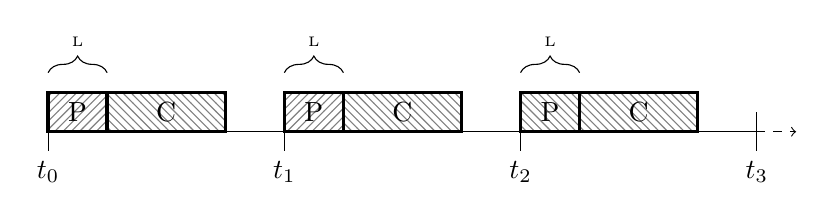
\begin{tikzpicture}[scale=0.5]
    \draw[] (6,0) -- (24,0);
    \draw[dashed, ->] (24,0) -- (25,0);
    \draw (6,0.5) -- (6,-0.5) node[below] {$t_{0}$};
    \draw (12,0.5) -- (12,-0.5) node[below] {$t_{1}$};
    \draw (18,0.5) -- (18,-0.5) node[below] {$t_{2}$};
    \draw (24,0.5) -- (24,-0.5) node[below] {$t_{3}$};

    \draw [pattern=north east lines, pattern color=gray, line width = 1pt, very thick] ($(6,0)$) rectangle ++($(1.5,1)$) node[midway] {P};
    \draw [pattern=north west lines, pattern color=gray, line width = 1pt, very thick] ($(7.5,0)$) rectangle ++($(3,1)$) node[midway] {C};
    \draw [decorate,decoration={brace,amplitude=6pt}]($(6,1.5)$) -- ++($(1.5,0)$) node [black,midway,above=6pt] {\tiny L};
    
    \draw [pattern=north east lines, pattern color=gray, line width = 1pt, very thick] ($(12,0)$) rectangle ++($(1.5,1)$) node[midway] {P};
    \draw [pattern=north west lines, pattern color=gray, line width = 1pt, very thick] ($(13.5,0)$) rectangle ++($(3,1)$) node[midway] {C};
    \draw [decorate,decoration={brace,amplitude=6pt}]($(12,1.5)$) -- ++($(1.5,0)$) node [black,midway,above=6pt] {\tiny L};
    
    \draw [pattern=north west lines, pattern color=gray, line width = 1pt, very thick] ($(18,0)$) rectangle ++($(1.5,1)$) node[midway] {P};
    \draw [pattern=north west lines, pattern color=gray, line width = 1pt, very thick] ($(19.5,0)$) rectangle ++($(3,1)$) node[midway] {C};
    \draw [decorate,decoration={brace,amplitude=6pt}]($(18,1.5)$) -- ++($(1.5,0)$) node [black,midway,above=6pt] {\tiny L};
\end{tikzpicture}

        \label{fig:correct_reconfig}
    } \\
    \subfloat[]{
        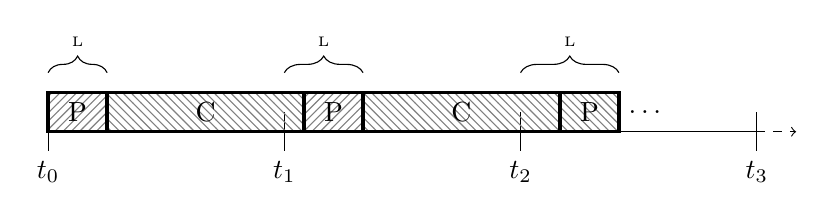
\begin{tikzpicture}[scale=0.5]
    \draw[] (6,0) -- (24,0);
    \draw[dashed, ->] (24,0) -- (25,0);
    \draw (6,0.5) -- (6,-0.5) node[below] {$t_{0}$};
    \draw (12,0.5) -- (12,-0.5) node[below] {$t_{1}$};
    \draw (18,0.5) -- (18,-0.5) node[below] {$t_{2}$};
    \draw (24,0.5) -- (24,-0.5) node[below] {$t_{3}$};

    \draw [pattern=north east lines, pattern color=gray, line width = 1pt, very thick] ($(6,0)$) rectangle ++($(1.5,1)$) node[midway] {P};
    \draw [pattern=north west lines, pattern color=gray, line width = 1pt, very thick] ($(7.5,0)$) rectangle ++($(5,1)$) node[midway] {C};
    \draw [decorate,decoration={brace,amplitude=6pt}]($(6,1.5)$) -- ++($(1.5,0)$) node [black,midway,above=6pt] {\tiny L};
    
    \draw [pattern=north east lines, pattern color=gray, line width = 1pt, very thick] ($(12.5,0)$) rectangle ++($(1.5,1)$) node[midway] {P};
    \draw [pattern=north west lines, pattern color=gray, line width = 1pt, very thick] ($(14,0)$) rectangle ++($(5,1)$) node[midway] {C};
    \draw [decorate,decoration={brace,amplitude=6pt}]($(12,1.5)$) -- ++($(2,0)$) node [black,midway,above=6pt] {\tiny L};
    
    \draw [pattern=north west lines, pattern color=gray, line width = 1pt, very thick] ($(19,0)$) rectangle ++($(1.5,1)$) node[midway] {P};
    % \draw [pattern=north west lines, pattern color=gray, line width = 1pt, very thick] ($(20.5,0)$) rectangle ++($(5,1)$) node[midway] {C};
    \draw [decorate,decoration={brace,amplitude=6pt}]($(18,1.5)$) -- ++($(2.5,0)$) node [black,midway,above=6pt] {\tiny L};
    \node[right] at (20.5,0.5) {\ldots};



\end{tikzpicture}
        \label{fig:incorrect_reconfig}
    }
    \caption{
    Example time lines of reconfiguration procedures.
    $t_n$ indicates the time instance where the $n$th frame has been received by the GrAICore, ready to be processed.
    At $t_0$, the GrAICore is already configured with an initial model.
    In \protect\subref{fig:correct_reconfig}, the GrAICore uses a different model for each consecutive frame.
    After receiving and processing (P) the very first frame at $t_0$, it starts reconfiguration (C) to a new model.
    Since the sum of the reconfiguration and processing time does not exceed the frame time ($t_{n+1} - t_{n})$, the frame processing latency (L) is equal for every incoming frame.
    The invariant latency is desired and indicates a seamless reconfiguration.
    \protect\subref{fig:incorrect_reconfig} has an increased reconfiguration time.
    Now, the sum of the reconfiguration and processing time does exceed the frame time.
    As a consequence, the frame processing latency increases for each incoming frame.
    In the long run, this latency will grow to infinity.
    Since the latency varies, this is an example of a non-seamless reconfiguration.
    }
    \label{fig:reconfig_time_line_ex}
\end{figure}

\subsubsection{Large model}

Due to the GrAICore having limited memory capacity, a single large model cannot be loaded onto it at once.
Several works have proposed strategies for deploying CNNs on resource-constrained devices.
Among these strategies, "partitioning" refers to splitting an entire model at specific locations to create one or more partitions, thereby reducing instantaneous memory requirements \cite{kaboubiHybridPartitioningEmbedded2023}.
To fully process a frame, one or more (partial) reconfigurations will need to be performed.
Each of the reconfigurations will load in the subsequent neural network part needed for further processing.

For this case, a specific timing or bandwidth cannot be as easily determined.
This is due to the nature of a large model. A large model can be of any arbitrary size.
With a larger model having to be partitioned into more parts.
Consequently, an increase in parts sees an increase in the amount of reconfigurations necessary to execute the large model completely.
Due to this, determining the total reconfiguration time budget is more involved.
A single frame is ``processed'' multiple times, once by each part of the neural network.
The total reconfiguration time budget is dependent on the number of (partial) reconfigurations necessary to fully process a single frame.

\begin{table}[hbtp]
\centering
\begin{tabular}{@{}lllllll@{}}
\toprule
    &            & \multicolumn{5}{l}{Time budget per reconfiguration amount (ms)} \\
FPS & Frame time (ms) & 1x         & 2x          & 3x         & 4x         & 5x         \\ \midrule
5   & 200  & 195  & 190  & 185  & 180   & 175   \\
15  & 66.7 & 61.7 & 56.7 & 51.7 & 46.7  & 41.7  \\
24  & 41.7 & 36.7 & 31.7 & 26.7 & 21.7  & 16.7  \\
30  & 33.3 & 28.3 & 23.3 & 18.3 & 13.3  & 8.3   \\
60  & 16.7 & 11.7 & 6.7  & 1.7  & -3.3  & -8.3  \\
120 & 8.3  & 3.3  & -1.7 & -6.7 & -11.7 & -16.7 \\ \bottomrule
\end{tabular}
\caption{Maximum reconfiguration time budget for common frame rates and different reconfiguration amounts. The frame times and time budgets are rounded.}
\label{tab:common_fps_reconfig_amount}
\end{table}

As an example, assume that a large model is partitioned into an arbitrary amount of parts.
Each part is exactly the size of the GrAICore's total capacity and the processing time for each part takes $\SI{5}{ms}$.
\Cref{tab:common_fps_reconfig_amount} shows that for a video of $\SI{60}{FPS}$ and a large model requiring two reconfigurations, we have a maximum reconfiguration time budget of $\SI{6.7}{ms}$.
Notice that a large model that requires $4$ reconfigurations at \SI{60}{FPS} has a negative time budget.
This means that it is not possible to process a frame for a video of \SI{60}{FPS} within two consecutive incoming frames for that particular model.
Processing frames at \SI{60}{FPS} with a large model is often not feasible, as many models require more than a few reconfigurations.
A lower frame rate gives us a larger reconfiguration budget, which is more suitable for larger models.
Notably, reducing the frame rate to single digits significantly increases the available reconfiguration budget.
\Cref{fig:larger_reconfig_ex} illustrates two time lines showing a good and a bad scenario.

\begin{figure}[htbp]
    \centering
    \subfloat[]{
        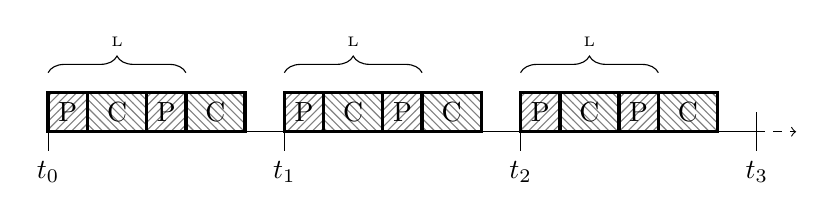
\begin{tikzpicture}[scale=0.5]

    \draw[] (6,0) -- (24,0);
    % \draw[dashed, <-] (5,0) -- (6,0);
    \draw[dashed, ->] (24,0) -- (25,0);
    \draw (6,0.5) -- (6,-0.5) node[below] {$t_{0}$};
    \draw (12,0.5) -- (12,-0.5) node[below] {$t_{1}$};
    \draw (18,0.5) -- (18,-0.5) node[below] {$t_{2}$};
    \draw (24,0.5) -- (24,-0.5) node[below] {$t_{3}$};
    
    \draw [pattern=north east lines, pattern color=gray, line width = 1pt, very thick] ($(6,0)$) rectangle ++($(1,1)$) node[midway] {P};
    \draw [pattern=north west lines, pattern color=gray, line width = 1pt, very thick] ($(7,0)$) rectangle ++($(1.5,1)$) node[midway] {C};
    \draw [pattern=north east lines, pattern color=gray, line width = 1pt, very thick] ($(8.5,0)$) rectangle ++($(1,1)$) node[midway] {P};
    \draw [pattern=north west lines, pattern color=gray, line width = 1pt, very thick] ($(9.5,0)$) rectangle ++($(1.5,1)$) node[midway] {C};
    \draw [decorate,decoration={brace,amplitude=6pt}]($(6,1.5)$) -- ++($(3.5,0)$) node [black,midway,above=6pt] {\tiny L};
    
    \draw [pattern=north east lines, pattern color=gray, line width = 1pt, very thick] ($(12,0)$) rectangle ++($(1,1)$) node[midway] {P};
    \draw [pattern=north west lines, pattern color=gray, line width = 1pt, very thick] ($(13,0)$) rectangle ++($(1.5,1)$) node[midway] {C};
    \draw [pattern=north east lines, pattern color=gray, line width = 1pt, very thick] ($(14.5,0)$) rectangle ++($(1,1)$) node[midway] {P};
    \draw [pattern=north west lines, pattern color=gray, line width = 1pt, very thick] ($(15.5,0)$) rectangle ++($(1.5,1)$) node[midway] {C};
    \draw [decorate,decoration={brace,amplitude=6pt}]($(12,1.5)$) -- ++($(3.5,0)$) node [black,midway,above=6pt] {\tiny L};
    
    \draw [pattern=north east lines, pattern color=gray, line width = 1pt, very thick] ($(18,0)$) rectangle ++($(1,1)$) node[midway] {P};
    \draw [pattern=north west lines, pattern color=gray, line width = 1pt, very thick] ($(19,0)$) rectangle ++($(1.5,1)$) node[midway] {C};
    \draw [pattern=north east lines, pattern color=gray, line width = 1pt, very thick] ($(20.5,0)$) rectangle ++($(1,1)$) node[midway] {P};
    \draw [pattern=north west lines, pattern color=gray, line width = 1pt, very thick] ($(21.5,0)$) rectangle ++($(1.5,1)$) node[midway] {C};
    \draw [decorate,decoration={brace,amplitude=6pt}]($(18,1.5)$) -- ++($(3.5,0)$) node [black,midway,above=6pt] {\tiny L};
\end{tikzpicture}

        \label{fig:large_reconfig_ex1}
    } \\
    \subfloat[]{
        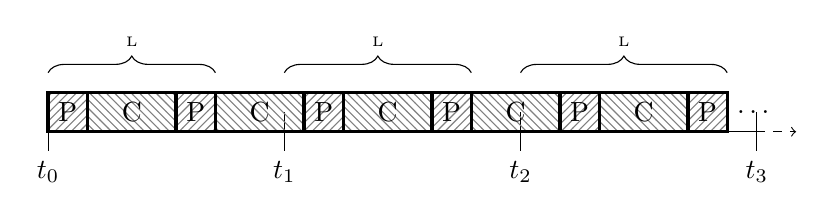
\begin{tikzpicture}[scale=0.5]

    \draw[] (6,0) -- (24,0);
    \draw[dashed, ->] (24,0) -- (25,0);
    \draw (6,0.5) -- (6,-0.5) node[below] {$t_{0}$};
    \draw (12,0.5) -- (12,-0.5) node[below] {$t_{1}$};
    \draw (18,0.5) -- (18,-0.5) node[below] {$t_{2}$};
    \draw (24,0.5) -- (24,-0.5) node[below] {$t_{3}$};
    
    \draw [pattern=north east lines, pattern color=gray, line width = 1pt, very thick] ($(6,0)$) rectangle ++($(1,1)$) node[midway] {P};
    \draw [pattern=north west lines, pattern color=gray, line width = 1pt, very thick] ($(7,0)$) rectangle ++($(2.25,1)$) node[midway] {C};
    \draw [pattern=north east lines, pattern color=gray, line width = 1pt, very thick] ($(9.25,0)$) rectangle ++($(1,1)$) node[midway] {P};
    \draw [pattern=north west lines, pattern color=gray, line width = 1pt, very thick] ($(10.25,0)$) rectangle ++($(2.25,1)$) node[midway] {C};
    \draw [decorate,decoration={brace,amplitude=6pt}]($(6,1.5)$) -- ++($(4.25,0)$) node [black,midway,above=6pt] {\tiny L};
    
    \draw [pattern=north east lines, pattern color=gray, line width = 1pt, very thick] ($(12.5,0)$) rectangle ++($(1,1)$) node[midway] {P};
    \draw [pattern=north west lines, pattern color=gray, line width = 1pt, very thick] ($(13.5,0)$) rectangle ++($(2.25,1)$) node[midway] {C};
    \draw [pattern=north east lines, pattern color=gray, line width = 1pt, very thick] ($(15.75,0)$) rectangle ++($(1,1)$) node[midway] {P};
    \draw [pattern=north west lines, pattern color=gray, line width = 1pt, very thick] ($(16.75,0)$) rectangle ++($(2.25,1)$) node[midway] {C};
    \draw [decorate,decoration={brace,amplitude=6pt}]($(12,1.5)$) -- ++($(4.75,0)$) node [black,midway,above=6pt] {\tiny L};
    
    \draw [pattern=north east lines, pattern color=gray, line width = 1pt, very thick] ($(19,0)$) rectangle ++($(1,1)$) node[midway] {P};
    \draw [pattern=north west lines, pattern color=gray, line width = 1pt, very thick] ($(20,0)$) rectangle ++($(2.25,1)$) node[midway] {C};
    \draw [pattern=north east lines, pattern color=gray, line width = 1pt, very thick] ($(22.25,0)$) rectangle ++($(1,1)$) node[midway] {P};
    % \draw [pattern=north west lines, pattern color=gray, line width = 1pt, very thick] ($(23.25,0)$) rectangle ++($(2.25,1)$) node[midway] {C};
    \node[right] at (23.25,0.5) {\ldots};
    \draw [decorate,decoration={brace,amplitude=6pt}]($(18,1.5)$) -- ++($(5.25,0)$) node [black,midway,above=6pt] {\tiny L};

\end{tikzpicture}
        \label{fig:large_reconfig_ex2}
    }
    \caption{
        Example time lines of processing a large model requiring two reconfigurations.
        At $t_0$, the GrAICore is already configured with the first part of the model.
        In \protect\subref{fig:large_reconfig_ex1}, the two reconfiguration periods (C) and two processing periods (P) fit within the reception of two consecutive frames ($t_n$ and $t_{n+1}$).
        The frame processing latency (L) is equal for every incoming frame.
        In \protect\subref{fig:large_reconfig_ex2}, the reconfiguration time is increased. 
        This results into an ever-increasing frame processing latency.
    }
    \label{fig:larger_reconfig_ex}
\end{figure}

We will examine realistic AI models, specifically the ResNet-101 model \cite{heDeepResidualLearning2015}, which is a potential use case for the GrAICore and exceeds its local memory, to understand the required timings and bandwidth.
This analysis will provide insights into the bandwidth requirements and power usage of a large AI model.
However, given the complexity of this analysis, it will be deferred to the project phase.

\subsubsection{Power consumption}
Since the GrAICore is primarily used as an AI accelerator for edge devices, maintaining low power consumption is crucial.
The addition of external memory with the capability to reconfigure the GrAICore will inevitably increase the overall power consumption of the system.
However, specific optimizations can be implemented to minimize this increase.
The solution should encompass the memory, interface, and controller, with a focus on achieving minimal power usage.

We are considering options such as DRAM or NVM, and the final selection will balance power efficiency, performance, and system compatibility.
It has been measured that the GrAICore consumes between \SI{200}{mW} and \SI{500}{mW} when processing frames at \SI{60}{FPS}.
We aim to not exceed \SI{20}{mW} when performing 60 reconfigurations per second.


% \section{Method}
% \section{Results and analysis}
% \section{Discussion}
% \section{Conclusions and future work}
% \subsection{Conclusions}
% \subsection{Future work}

% % \section{Evaluation of the config Noc}
% \section{Introduction}
The config NoC is mainly used for configuration writes to the neuron core memories.
Another use is status monitoring reads while the GrAICore is in operation.
The config NoC is a separate NoC next to the event NoC, which is used for the execution of a model.
It connects all 144 neuron cores via a 2D mesh topology (see \cref{fig:noc}).
The network receives and forwards data using routers at each neuron core.
The config NoC has a single 16-bit wide interface for incoming data from an AXI slave.
Similarly, the links between every two adjacent routers are 16-bit wide. 
The clock frequency of the system is \SI{800}{MHz}.


\section{Architecture}
\lipsum[1]
% purpose
% topology
% 
The config NoC makes u
The config NoC incorporates a 2D 
Unlike the event NoC, the config NoC incorporates a 2D mesh topology.
The wraparound links of the event NoC provide noticeable benefits in communication performance.
In the event NoC, intercommunication happens between the neuron cores.
The presence of the wraparound links helps to drastically reduce the average amount of hops a packet has to take.
T
The wraparound links do not provide any noticeable benefits to the config NoC since these interactions do not occur with the config NoC.


\section{Network packet format}
The network makes use of network packets for data communication.
The phit size of the config NoC is 16 bits wide.
This implies that a total of 16 bits of data can be transferred over a link in a single cycle.
Each packet contains a header, made up of two separate phits.
The header contains the fields as shown in \cref{tab:header_fields}.

\begin{table}[hbtp]
\centering
\begin{tabular}{@{}ll@{}}
\toprule
\textbf{Header field} & \textbf{\# of bits} \\ \midrule
Packet type           & 2                   \\
Destination cluster X & 4                   \\
Destination cluster Y & 4                   \\
Address               & 20                  \\ \bottomrule
\end{tabular}
\caption{Header fields of a config NoC packet}
\label{tab:header_fields}
\end{table}

The \textit{packet type} field defines whether the packet is a \textit{read request}, \textit{read response} or \textit{write request} packet.
A \textit{read request} packet is initiated by the host.
It is used to retrieve data from a neuron core.
A \textit{read response} packet is produced as an answer to a \textit{read request}.
This packet contains the requested data that is sent back to the host.
Finally, the \textit{write request} is used to write data to a neuron core.

Both the \textit{read response} and \textit{write request} packets has two phits following the header (see \cref{fig:read_response_packet,fig:write_request_packet}).
These two phits contain the payload data that is requested.
Thus in total, packets of these two types are 64 bits in size.
The \textit{read request} packet only consists of the header (see \cref{fig:read_request_packet}).

The destination cluster coordinates are both 4 bits in size due to the need to address 12 different X and 12 different Y coordinates.

The \textit{address field} of 20 bits, allows the system to address $2^{20}$ different addresses.
This address space is used to address the SRAM and the register bank of a neuron core.
% This address space is used to address the SRAM and the register bank of a neuron core, with room to spare \cite{TODO}.

With this packet format, we observe that there is a significant overhead when writing or reading data.
For every 32 bits of data we read or write, an overhead of 32 bits is also included.
In other words, there is an overhead of $100\%$ for every read or write request of 32 bits.
At most, on average, the network transmits one byte of payload data per cycle.

% There is potential to increase this to 64 bits (or 8 bytes) per cycle which is the amount of data an SRAM in a single core can write in a single cycle.

\hspace*{0.5em}
\begin{figure}[htbp]
    \centering
    \begin{subfigure}[b]{\linewidth}
        \centering
        \begin{adjustbox}{width=0.8\linewidth}
            \input{assets/packet_format/read_request_packet}
        \end{adjustbox}
        \caption{Read request}
        \label{fig:read_request_packet}
    \end{subfigure}
    \\ \vspace{1.5em}
    \begin{subfigure}[b]{\linewidth}
        \centering
        \begin{adjustbox}{width=0.8\linewidth}
            \input{assets/packet_format/read_response_packet}
        \end{adjustbox}
        \caption{Read response}
        \label{fig:read_response_packet}
    \end{subfigure}
    \\ \vspace{1.5em}
    \begin{subfigure}[b]{\linewidth}
        \centering
        \begin{adjustbox}{width=0.8\linewidth}
            \begin{bytefield}[
    boxformatting={\centering\ttfamily},
    bitformatting={\ttfamily\small},
    endianness=big,
    bitwidth=2em
]{16}
\bitheader{0, 2, 6, 10, 12, 15} \\

\begin{rightwordgroup}{Header}
    \bitbox{4}[bgcolor=lightcyan]{Address[3:0]} &
    \bitbox{2}[bgcolor=lightgray]{Unused} &
    \bitbox{4}[bgcolor=lightred]{Dest. Y} &
    \bitbox{4}[bgcolor=lightorange]{Dest. X} &
    \bitbox{2}[bgcolor=lightgreen]{\scriptsize Packet type} \\

    \bitbox{16}[bgcolor=lightcyan]{Address[19:4]}
\end{rightwordgroup} \\

\begin{rightwordgroup}{Payload}
    \bitbox{16}[bgcolor=lightpurple]{Write data[15:0]} \\
    \bitbox{16}[bgcolor=lightpurple]{Write data[31:16]}
\end{rightwordgroup}

\end{bytefield}
        \end{adjustbox}
        \caption{Write request}
        \label{fig:write_request_packet}
    \end{subfigure}
    \caption{
        Config NoC packet structures
    }
    \label{fig:config_noc_packets}
\end{figure}

\section{Bandwidth}
Configuration is done by transferring write request packets from the host to one or more neuron cores.
A write request packet consists of 64 bits in total.
Recall that the SRAM capacity of a single neuron core is \SI{256}{KiB}.
If we want to completely fill up one of these memories, a total of $\frac{\SI{256}{KiB}}{\SI{32}{b}} = 65536$ write request packets needs to be sent.
This means that, in total, \SI{256}{KiB} of payload data and \SI{256}{KiB} of header data is sent through the NoC.

To estimate the time to write a certain amount of data to the memories of the GrAICore, we can make use of \cref{eq:latency}.
The effective bandwidth can be calculated with \cref{eq:bandwidth}.

\begin{equation}
    T = 
    \frac{d_{\text{payload}} + d_{\text{overhead}}}
    {f_{\text{clock}} \times w_{\text{phit}}}
\label{eq:latency}
\end{equation}

\begin{equation}
    \text{BW}_{\text{eff}} =
    \frac{d_\text{payload}}{T}
\label{eq:bandwidth}
\end{equation}

\begin{eqexpl}[15mm]
    \item{$T$} time to write data
    \item{$\text{BW}_{\text{eff}}$} effective bandwidth
    \item{$d_{\text{payload}}$} amount of payload data
    \item{$d_{\text{overhead}}$} amount of overhead data
    \item{$f_{\text{clock}}$} system's clock frequency
    \item{$w_{\text{phit}}$} width of a phit
\end{eqexpl}

For example, to completely fill up the GrAICore's memory (\SI{36}{MiB}), it will take around \SI{47}{ms}\footnote{$\frac{\SI{36}{MiB} + \SI{36}{MiB}}{\SI{800}{MHz} \times \SI{16}{b}}$}.
% This translates to an effective bandwidth of $\frac{\SI{36}{MiB}}{\SI{47}{ms}} \approx \SI{763}{MiB/s}$.
This translates to an effective bandwidth of \SI{763}{MiB/s}\footnote{$\frac{\SI{36}{MiB}}{\SI{47}{ms}}$}.
Here we assumed that no delays are introduced by software and reading the data from storage.
Furthermore, it is good to note that the delays introduced by hops are minimal due to pipelining.
Thus, \cref{eq:bandwidth} provides us the config NoC's \textit{peak} effective bandwidth.
% \include{sections/multiple_models_analysis}
% \include{sections/large_model_analysis}
% This section discusses various modifications to the config NoC that can be implemented to improve the configuration speed of the GrAICore.

% TODO add introduction to chapter
\lipsum[1]
% \section{Proposed specifications}
\label{sec:proposed_noc}
To improve the bandwidth of configuration with the \confignoc{}, a set of changes is proposed. Firstly, we propose to widen the links from 16 bits to 64 bits.
This allows for phits of 64 bits in size.
This change provides us with a potential bandwidth increase of 4x.
An immediate increase to 64 bits instead of 32 bits is preferred as it allows for one-time change in the design and verification effort.
Another benefit is the synergy with the unified memories.
Since the SRAMs have 64-bit memory words and can write one memory word of 64 bits every cycle, there is no need to buffer multiple (smaller) phits before writing them to the SRAM.
This first change proposal provides a peak bandwidth of \SI{3}{GiB/s}.

Next, by dividing the \confignoc{} into two equally sized (virtual) zones with their own external interface, we can benefit from parallel configuration of two cores (one per zone) and therefore, another 2x increase in bandwidth.
These two changes provide a bandwidth of around \SI{6}{GiB/s}. 
The amount of zones and injection points can be expanded in the future at relatively small costs if necessary.

Lastly, the aforementioned changes require a change in the packet format.
The new packet format benefits from less overhead per chunk of payload data.
Since we opt for a link width of 64, the size of a single phit also increases to 64 bits.
All header information fits within a single phit of 64 bits.
The data phits following the header are fully utilized for payload data.
The format of the header is shown in \cref{fig:packet_format_header_new}.
With a length field of 6 bits, we can specify up to 64 data phits for a single packet.
This is a sufficient amount as argued in the previous section. 
Compared to the current packet format, an additional bandwidth increase of almost 2x can be gained with this new packet format.

\begin{figure}[hbtp]
    \centering
    \resizebox{\linewidth}{!}{
        \newcommand{\fakesixtyfourbits}[1]{%
    \ttfamily
    \small
    \ifnum#1=1234567890
        #1
    \else
        \ifnum#1=40
            % \count32=#1
            % \advance\count32 by 48
            % \the\count32%
            63%
        \else
            \ifnum#1<37
                #1%
            \else
                \ifnum#1=38
                    $\cdots$%
                \fi
            \fi
        \fi
    \fi
}

\begin{bytefield}[
    boxformatting={\centering\ttfamily},
    % bitformatting={\ttfamily\small},
    bitformatting={\fakesixtyfourbits},
    endianness=big,
    bitwidth=1.5em,
    bitheight=2.5em
]{41}
% \bitheader{0-45} \\
\bitheader{40, 38, 36, 30, 10, 6, 2, 0} \\

\bitbox{5}[bgcolor=lightgray]{Unused} &
\bitbox{6}[bgcolor=lightyellow]{Length[5:0]} &
\bitbox{20}[bgcolor=lightcyan]{Address[19:0]} &
\bitbox{4}[bgcolor=lightred]{Dest. Y} &
\bitbox{4}[bgcolor=lightorange]{Dest. X} &
\bitbox{2}[bgcolor=lightgreen]{\scriptsize Packet type} \\

\end{bytefield}
    }
    \caption{Proposed packet header format}
    \label{fig:packet_format_header_new}
\end{figure}

Through increasing the link width, adding an additional injection point, and adopting a new packet format, it's possible to achieve a significant peak bandwidth improvement of nearly 16x.
Specifically, this translates to upgrading from an initial effective write bandwidth of \SI{763}{MiB/s} to a substantial \SI{11.92}{GiB/s}.
Moreover, additional increase in bandwidth can be obtained by increasing the amount of injection points.

% To obtain an insight into the power consumption with the introduction of the config NoC changes in \cref{TODO} and model configuration using external memory we will provide an comprehensive analysis.
% To get an approximation of the power consumption when configuring the GrAICore with a model and processing frames with it, we will provide calculations with energy parameters acquired from internal sources.

When configuring the GrAICore and processing an input frame, the major components that consume energy are as follows:
\begin{itemize}
    \item Configuration
    \begin{itemize}
        \item Reading data from the external memory
        \item Transferring data from the external memory to the config NoC
        \item Phits traversing (i.e., hops) through the config NoC
        \item Writing data to the neuron core's SRAM
    \end{itemize}
    \item Processing
    \begin{itemize}
        \item Processing the input frame by the model
    \end{itemize}
\end{itemize}

\section{Configuration energy}
Since we have access to various energy parameters for DDR memory, we will use DDR memory as an example.

\begin{figure}[hbtp]
    \centering
    \includegraphics[width=0.8\linewidth]{assets/ddr_graicore_block_diagram.pdf}
    \caption{
        Interconnection of the DDR device and GrAICore
    }
    \label{fig:ddr_graicore_block_diagram}
\end{figure}

A typical system with DDR as external memory looks as shown in \cref{fig:ddr_graicore_block_diagram}.
% TODO add image
\begin{itemize}
    \item The \textit{DDR device} where the (model) data is read from.
    \item The \textit{DDR PHY} that connects the \textit{DDR device} and \textit{DDR controller}.
    \item The \textit{DDR controller} that handles the read/write requests from the \textit{GrAICore}.
    \item The \textit{AXI bus} that connects the \textit{DDR controller} and \textit{GrAICore}.
    \item The \textit{GrAICore} that transfers and writes data the SRAMs.
\end{itemize}

% It has been established that performing a hop on the Event NoC consumes around \SI{129}{fJ}.
% These hops are for phits of 32 bits.
% For the Config NoC (which uses phits of 16 bits), we are interested in the energy use for transferring phits of 16 bits. We can approximate this value by dividing the value for 32 phit hops into two. I.e., 129 fJ / 2 = 64.5 fJ. 

% Furthermore, it has been established that for the SRAM to write 64 bits, it consumes \SI{2.490}{pJ}.
% The SRAM system has the property to write 64 bits at once by first buffering four consecutive phits.
% This improves efficiency. 

For the analysis, we assume that we are using the newly proposed config NoC in \cref{sec:proposed_noc}. 
With the new packet format, a packet contains at most 65 data phits of 64 bits each.
That is, a maximum of 520 bytes\footnote{$65 \times \frac{\SI{64}{b}}{8} = \SI{520}{B}$} of payload per packet.
Furthermore, an additional injection point is introduced (see \cref{fig:segmentation_example_2}).
Next to the injection point connected to the router on the bottom left of the config NoC, a new one is added and connected to the router six positions up.

To estimate the energy cost for configuration, we require the following information from a model:
\begin{itemize}
    % \item Amount of data to read from the external memory
    \item Amount of data to transfer to the SRAMs
    \item Core destination of the data
\end{itemize}

The amount of data to transfer determines how much data will be read, transferred and written.
We are assuming that the same amount of data read from the external memory is written to the SRAMs.
The location (specific neuron core) of the data determines the amount of hops the data has to perform in the config NoC.
The amount of data to write can also be used to determine the configuration time.
The configuration time is calculated by dividing the amount of data with the write bandwidth.
The configuration time is used for computing the energy for the \textit{DDR PHY}, \textit{DDR controller} and \textit{AXI bus}.

The amount of data to be written and to which neuron cores depends on how the compiler has performed the mapping on the GrAICore. % explain
Phits that needs to be transferred to neuron cores further away from an injection point will require more hops to reach, and therefore consume more energy than neuron cores closer to an injection point.
The amount of data that needs to be written to each core differs.
We can retrieve this information from the compiler.

For estimating the energy for the GrAICore component, we consider the config NoC and the SRAMs.
The config NoC consumes energy by transferring the phits to its destinations via one or multiple hops through the NoC.
The SRAM consumes energy by writing the data to its banks.
A single hop through the config NoC with a 64 bit phit consumes \SI{0.258}{pJ}.
Writing back 64 bits to an SRAM consumes \SI{4.980}{pJ}.

\begin{table}[hbtp]
\centering
\begin{tabular}{@{}lll@{}}
\toprule
\textbf{Component}      & \textbf{Usage}  &  \\
\midrule
DDR device              & \SI{0.11}{nJ/B} &  \\
DDR PHY                 & \SI{133}{mW}    &  \\
DDR controller          & \SI{20}{mW}     &  \\
AXI bus                 & \SI{80}{mW}     &  \\
NoC hop (\SI{64}{b})    & \SI{0.258}{pJ}  &  \\
SRAM write (\SI{64}{b}) & \SI{4.980}{pJ}  &  \\
\bottomrule
\end{tabular}
\caption{Energy parameters for each of the major energy consuming components. The shown power numbers for \textit{DDR PHY}, \textit{DDR controller} and \textit{AXI bus} are when at full capacity (i.e., best-case scenario).}
\label{tab:energy_parameters_ddr}
\end{table}

\subsection{Calculation}
The configuration energy consists of the reading, transferring and writing of data from the external memory to the GrAICore's SRAMs. 

Let $C$ be the set of tuples holding the coordinates of every core:
\begin{equation*}
    C = \{\,\left(x,y\right) \in \mathbb{N}^2 \mid 1 \leq x \leq 12 \wedge 0 \leq y \leq 11 \,\} 
\end{equation*}

Notice that the x-coordinate and y-coordinate starts at index $1$ and $0$ respectively.

\Cref{fig:model_data_heapmap} shows for a $80\%$ pruned version of ResNet-50\footnote{Internally named \texttt{resnet50\_pruned80\_star}} the amount of data that needs to be written to each of the 144 neuron cores.
We observe that the data is not uniformly distributed across the SRAMs.
Therefore, we require information how much data needs to be transferred to each SRAM.

\begin{figure}[hbtp]
    \centering
    \includegraphics[width=0.8\linewidth]{assets/model_data_heatmap.png}
    \caption{Amount of data to be written to each core for the ResNet-50 model (80\% pruned).}
    \label{fig:model_data_heapmap}
\end{figure}

Let $D$ be a matrix of $12 \times 13$ with $D_{i,j}$ denoting the amount of bytes to be written to core $\left( i,j \right)$.
$D$ has an additional column due to the x-coordinates not starting from index $0$.
Its left-most column is unused (i.e., $D_{0,0}, D_{0,1}, \cdots, D_{0,11}$).
This matrix can be constructed from the artifacts outputted by the compiler.

The number of phits to be transferred through the config NoC influences the total energy costs.
In particular, the amount of phits to be transferred affects the number of hops to be taken in total and the amount of data to be written to the SRAMs.
Therefore, we need to determine how many phits needs to be transferred to each neuron core.
% The number of phits to be transferred influences the energy cost in the config NoC hops and SRAM writes.
% A packet can contain up to 520 bytes\footnote{$65 \times \frac{64}{8}$} of payload data. 
A packet can contain up to 65 data phits, that is $65 \times \SI{64}{b} = \SI{520}{B}$ of payload data.
% If we transfe
Suppose we need to transfer $d$ bytes to a neuron core, we then require a total of $\left\lfloor \frac{d}{520} \right\rfloor$ packets with 65 data phits.
% If $d \bmod 520 > 0$, then there is an additional packet consisting of $\left\lceil \frac{\left( d \bmod 520 \right) \times 8}{64}\right\rceil$ data phits.
If $\left( d \bmod 520 \right) > 0$, then there is an additional packet for the remaining $\left( d \bmod 520 \right)$ bytes of data.
The remaining packet will consist of $\left\lceil \frac{d \bmod 520}{8}\right\rceil$ data phits.
Note that each packet also contains a single phit of 64 bits for the header information.

The total energy cost for configuring the GrAICore can be estimated with the following equation:
\begin{equation}
    E_{\textrm{config}} = E_{\textrm{ext\_mem}} + E_{\textrm{noc}} + E_{\textrm{write}}
\end{equation}

With:
\begin{align*} 
E_{\textrm{ext\_mem}} &= 
        \sum_{c \in C}^{}{E_\textrm{read\_ext\_mem}(D_c) + E_{\textrm{send\_to\_noc}}(D_c)} \\
E_{\textrm{noc}} &=
    E_{\textrm{hop}} \times \sum_{c \in C}^{}{N_\textrm{hops}(c) \times p_{\textrm{total}}(D_c)} \\
E_{\textrm{write}} &=
    E_{\textrm{sram\_write\_64b}} \times \sum_{c \in C}^{}{p_{\textrm{data}}(D_c)}
\end{align*}

And:
\begin{align*} 
N_{\textrm{hops}}(x,y) &=
    \begin{cases} 
        x + y & \textrm{if } 0 \leq y \leq 5 \\
        x + y - 6 & \text{if } 6 \leq y \leq 11
    \end{cases}
\\
p_{\textrm{total}}(d) &=
    \left\lfloor \frac{d}{520} \right\rfloor \times (65 + 1) + \left\lceil \frac{d \bmod 520}{8} \right\rceil + 1 =
    \left\lceil \frac{d}{8} \right\rceil + \left\lfloor \frac{d}{520} \right\rfloor + 1 
\\
p_{\textrm{data}}(d) &=
    \left\lfloor \frac{d}{520} \right\rfloor \times 65 + \left\lceil \frac{d \bmod 520}{8} \right\rceil =
    \left\lceil \frac{d}{8} \right\rceil
\end{align*}

\begin{eqexpl}[15mm]
    \item{$p_{\textrm{total}}(D_c)$} total phits (includes headers) for transferring $D_c$ bytes
    \item{$p_{\textrm{data}}(D_c)$} total data phits (excludes headers) for transferring $D_c$ bytes
    \item{$N_{\textrm{hops}}(c)$} the amount of hops required to reach a neuron core at coordinate $c$, starting from the router closest to the injection point. It has two sub-functions due to the new config NoC's dual injector architecture
    \item{$E_{\textrm{read\_ext\_mem}}(D_c)$} energy for reading $D_c$ bytes from the external memory
    \item{$E_{\textrm{send\_to\_noc}}(D_c)$} energy for sending $D_c$ bytes from the external memory to the config NoC
    \item{$E_{\textrm{hop}}$} energy for performing a single hop in the config NoC
    \item{$E_{\textrm{sram\_write\_64b}}$} energy for writing back 64 bits to a neuron core's SRAM
\end{eqexpl}

\section{Processing energy}
The processing energy is the energy consumed when the GrAICore is processing input frames.
% Note that the GrAICore does not make use of the config NoC to process input frames.
Note that the GrAICore uses the event NoC for communication between nodes when processing input frames, the config NoC is not involved in this process.

The processing energy can be estimated with the following equation:
\begin{equation}
    E_{\textrm{frame}} = \textrm{avg\_util} \times \textrm{cores\_used} \times \textrm{processing\_latency} \times \SI{21}{mW}
\end{equation}

These parameters can be obtained by simulating the model with \textit{GrAIPEFRUIT}, an in-house simulator for estimating inference performance.
Processing latency (\textrm{processing\_latency}) is the time the model takes to fully process a single frame, from input to output.
Cores used (\textrm{cores\_used}) is the amount of neuron cores that were used to execute the model.
Average utilization (\textrm{avg\_util}) is the average percentage of the time the cores were active while the frame was processed. 
The constant \SI{21}{mW} is the approximated power usage of a single neuron core while it's being fully utilized.
This constant is obtained from internal RTL simulations.

Since the config NoC is not involved in the processing of an input frame, any change to the config NoC does not influence the processing energy.
A significant factor (other than hardware changes) that may affect the processing energy is the mapping performed by the compiler on the original model. 
Different mappings on the same model have an effect on the average utilization and the number of neuron cores used, which in turn influences the processing latency.

\section{Evaluation}
To develop a preliminary understanding of the power contributions of the model reconfiguration from external memory, we evaluate a variety of practical models.
The power is the configuration of a model and a single inference with the model at \SI{60}{FPS}.
Effectively, this means that the same model is configured on the GrAICore 60 times per second and also used to proces an input frame 30 times per second.

We will be looking at two different external memory technologies, LPDDR5X and PCM.
We assume we use the DDR protocol for transferring data to the AXI bus that is connected to the GrAICore.
For the DDR protocol to work, we require an DDR PHY and DDR controller.
These components both add to the energy when transferring data to the GrAICore.

\begin{table}[hbtp]
    \centering
    \begin{tabular}{@{}lrl@{}}
    \toprule
    \textbf{Component} & \textbf{Value} & \textbf{Unit} \\
    \midrule
    LPDDR5X read             & 36.00 & pJ/B \\
    PCM read                 & 5.29 & pJ/B  \\
    DDR PHY                  & 10.39 & pJ/B \\
    DDR Controller           & 1.56 & pJ/B  \\
    AXI Bus                  & 6.25 & pJ/B  \\
    Config NoC hop (64 bits) & 0.26 & pJ    \\
    SRAM write (64 bits)     & 4.98 & pJ    \\ \bottomrule
    \end{tabular}
    \caption{Energy parameters of PCM and LPDDR5X memory, DDR interface and GrAICore that are relevant for model configuration}
    \label{tab:energy_parameters}
\end{table}

We look at the models as shown in \cref{tab:example_models_stats}.
It also shows the processing latency, the number of cores used and the average utilization of the cores of each (mapped) model.
These statistics are used for computing the processing energy.
The ``to write'' columns show the total amount of bytes that is to be transferred to the GrAICore.
Note that to get a more accurate energy number for configuration, we need the amount of bytes to be transferred to each core individually.
This information is available, and will be used for the evaluation.

\begin{table}[]
\centering
\begin{tabular}{@{}lrrrrr@{}}
\toprule
\textbf{Model}          & \textbf{\begin{tabular}[c]{@{}l@{}}Latency\\ (ms)\end{tabular}} & \textbf{Cores} & \textbf{Avg util.} & \textbf{\begin{tabular}[c]{@{}l@{}}To write\\ (MiB)\end{tabular}} \\ \midrule
efficientnet            & 1.642                                                           & 144            & 50.89\%            & 16.15                                                             \\
mobnetv2                & 1.296                                                           & 144            & 40.78\%            & 10.67                                                             \\
hand\_tracker           & 1.480                                                           & 144            & 36.62\%            & 12.33                                                             \\
hand\_detector          & 4.809                                                           & 144            & 68.03\%            & 19.12                                                             \\
resnet50                & 5.765                                                           & 144            & 36.35\%            & 29.58                                                             \\
resnet101\_p0           & 7.080                                                           & 144            & 33.40\%            & 28.75                                                             \\
resnet101\_p1           & 2.647                                                           & 143            & 36.42\%            & 20.06                                                             \\
resnet101\_p2           & 4.011                                                           & 144            & 33.12\%            & 30.44                                                             \\
resnet101\_p3           & 2.343                                                           & 143            & 33.55\%            & 17.71                                                             \\
resnet101\_p4           & 2.040                                                           & 143            & 26.19\%            & 15.54                                                             \\
resnet101\_pruned\_p0   & 6.552                                                           & 144            & 38.10\%            & 15.87                                                             \\
resnet101\_pruned\_p1   & 3.245                                                           & 143            & 34.31\%            & 10.43                                                             \\
resnet101\_pruned\_p2   & 4.501                                                           & 143            & 33.83\%            & 16.00                                                             \\
resnet101\_pruned\_p3   & 2.114                                                           & 143            & 38.08\%            & 10.22                                                             \\
resnet101\_pruned\_p4   & 2.437                                                           & 143            & 24.25\%            & 7.69                                                              \\
\bottomrule
\end{tabular}
\caption{Model statistics}
\label{tab:example_models_stats}
\end{table}

As an example, we demonstrate a calculation for the ResNet-50 model.
The processing energy is calculated as follows:
\begin{equation}
    E_\textrm{proc} = 0.3635 \times 144 \times \SI{5.765}{ms} \times \SI{21}{mW} = \SI{6.34}{mJ}
\end{equation}

\Cref{fig:model_data_heapmap} shows for the mapped ResNet-50 the amount of data to be sent to each individual core.
We use this information to construct matrix $D$ and the configuration energy $E_\textrm{conf}$.
We obtain the values as shown in \cref{tab:resnet50_energy}.
Configuration with LPDDR5X of the ResNet-50 model on the GrAICore consumes \SI{1.71}{mJ} and with PCM \SI{0.76}{mJ}.

\begin{table}[hbtp]
    \centering
    \begin{tabular}{@{}ll@{}}
    \toprule
    \textbf{Component} & \textbf{Value} \\
    \midrule
    $\ereadlpddr5x$ & 1116.8 \\
    $\ereadpcm$ & 164.2 \\
    $\ephy$ & 322.4 \\
    $\ectrl$ & 48.5 \\
    $\eaxi$ & 193.9 \\
    $\enoc$ & 9.2 \\
    $\ewrite$ & 19.3 \\
    \bottomrule
    \end{tabular}
    \caption{All values are in \SI{}{\micro\joule}}
    \label{tab:resnet50_energy}
\end{table}

% Then, performing a single configuration and a single inference, the system will consume \SI{8.05}{mJ} for LPDDR5X and \SI{7.09}{mJ} for PCM in total.
Then, the total energy consumption when performing a single configuration and a single inference is \SI{8.05}{mJ} for LPDDR5X and \SI{7.09}{mJ} for PCM.

\begin{figure}[hbtp]
    \centering
    \subcaptionbox{LPDDR5X\label{fig:pie_resnet50_conf_lpddr5x}}{
        \import{assets/power_analysis}{pre}
\begin{tikzpicture}
    \pie[
        radius=1.8,
        text=pin,
        color = {blue!60, blue!50, blue!40, blue!30, blue!20, blue!10},
        before number=\printonlylargeenough{10},
        after number=\ifprintnumber\%\fi
    ]{
        % 64.9/$\eread$,
        % 19.3/$\ephy$,
        % 2.8/$\ectrl$,
        % 11.3/$\eaxi$,
        % 0.5/$\enoc$,
        % 1.1/$\ewrite$
        64.9/$\eread$,
        19.3/$\ephy$,
        % 2.8/$\ectrl$,
        11.3/$\eaxi$,
        % 0.5/$\enoc$,
        % 1.1/$\ewrite$
        4.4/$\textrm{other}$
    }
\end{tikzpicture}

    }
    \hfill
    \subcaptionbox{PCM\label{fig:pie_resnet50_conf_pcm}}{
        \import{assets/power_analysis}{pre}
\begin{tikzpicture}
    \pie[
        radius=1.8,
        text=pin,
        color = {blue!60, blue!50, blue!40, blue!30, blue!20, blue!10},
        before number=\printonlylargeenough{10},
        after number=\ifprintnumber\%\fi
    ]{
        % 21.4/$\eread$,
        % 43.3/$\ephy$,
        % 6.3/$\ectrl$,
        % 25.3/$\eaxi$,
        % 1.2/$\enoc$,
        % 2.5/$\ewrite$
        21.4/$\eread$,
        43.3/$\ephy$,
        % 6.3/$\ectrl$,
        25.3/$\eaxi$,
        10.0/$\textrm{other}$
        % 1.2/$\enoc$,
        % 2.5/$\ewrite$
    }
\end{tikzpicture}

    }
    \caption{ResNet-50 configuration energy distribution}
    \label{fig:resnet50_conf_energy_distribution}
\end{figure}

% \Cref{TODO} shows that for LPDDR5X memory, reading from the memory consumes most of the energy in the configuration process.
% While the DDR PHY consumes the most energy when PCM is used.

Looking at the configuration energy, with LPDDR5X, most of the energy is consumed by reading from the exteral memory (see \cref{fig:resnet50_conf_energy_distribution}).
While for PCM, most of the energy is consumed by the DDR PHY.

The energy distribution between configuration and processing.
Shown in \cref{fig:resnet50_conf_proc}, the configuration of the ResNet-50 model occupies around 21\% with LPPDDR5X and 11\% with PCM of the total energy consumption (processing and configuration).
Of the models as listed in \cref{tab:example_models_stats}, on average, around 23\% is used for configuration with LPDDR5X memory and 12\% with PCM as external memory (see \cref{fig:example_models_avg_conf_proc}).
When performing configuration and processing at \SI{60}{FPS}, we get the power values as shown in \cref{tab:example_models_power_consumption}.

Ideally, the power consumption of the configuration of a model should be as minimal as possible.
In \cref{chapter:model_configuration_improvements}, we explore techniques for increasing configuration efficiency.

\begin{table}[]
    \centering
    \begin{threeparttable}
        \begin{tabular}{@{}lrrr@{}}
            \toprule
                                       & \multicolumn{2}{l}{\textbf{Conf. power (mW)}} & \textbf{Proc. power (mW)} \\ \cmidrule(l){2-3} 
            \textbf{Model}             & \textit{LPDDR5X}  & \textit{PCM}    & \\ \midrule
            efficientnet               & 56.0              & 24.8            & 151.6 \\
            mobnetv2                   & 37.0              & 16.4            & 95.9 \\
            hand\_tracker              & 42.8              & 18.9            & 98.3 \\
            hand\_detector             & 66.3              & 29.4            & 593.6 \\
            resnet50                   & 102.6             & 45.4            & 380.2 \\
            resnet101\tnote{1}         & 390.2             & 172.8           & 1081.7 \\
            resnet101\_pruned\tnote{1} & 208.9             & 92.5            & 1179.4 \\ \bottomrule
        \end{tabular}
        \begin{tablenotes}
            \item[1] Combination of all parts
        \end{tablenotes}
    \end{threeparttable}
    \caption{Power consumption of configuration (of the same model) and processing of an input frame at \SI{60}{Hz}}
    \label{tab:example_models_power_consumption}
\end{table}

\begin{figure}[hbtp]
    \centering
    \subcaptionbox{LPDDR5X\label{fig:pie_resnet50_conf_proc_lpddr5x}}{
        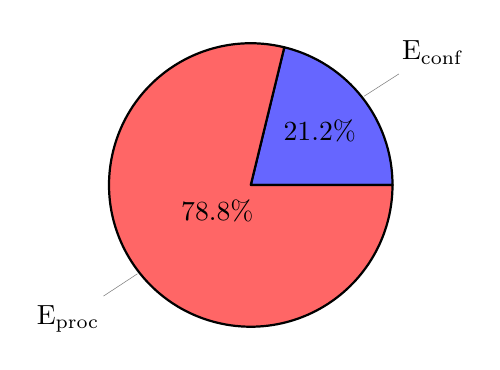
\begin{tikzpicture}
    \pie[
        radius=1.8,
        text=pin,
        color={blue!60, red!60},
    ]{
        21.2/$\econf$,
        78.8/$\eproc$
    }
\end{tikzpicture}

    }
    \hfill
    \subcaptionbox{PCM\label{fig:pie_resnet50_conf_proc_pcm}}{
        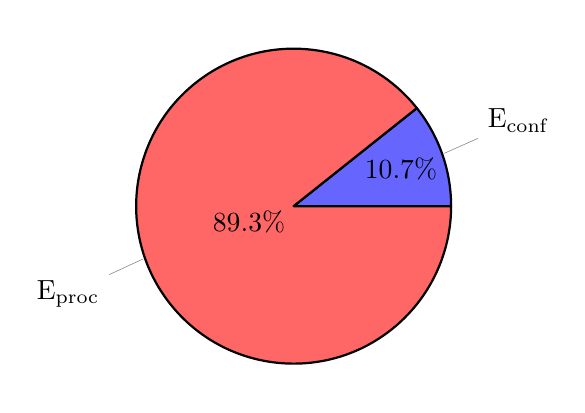
\begin{tikzpicture}
    \pie[
        radius=2,
        text=pin,
        color={blue!60, red!60},
    ]{
        10.7/$\econf$,
        89.3/$\eproc$
    }
\end{tikzpicture}

    }
    \caption{Configuration vs. processing energy for the ResNet-50 model}
    \label{fig:resnet50_conf_proc}
\end{figure}

\begin{figure}[hbtp]
    \centering
    \subcaptionbox{LPDDR5X\label{fig:sunburst_avg_conf_proc_lpddr5x}}{
        \import{assets/power_analysis}{pre}
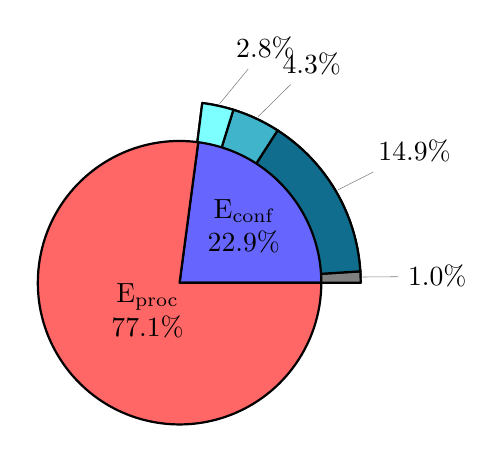
\begin{tikzpicture}
    \pie[
        radius=2.3,
        text=pin,
        hide number,
    ]{
        1.0/1.0\%,
        14.9/14.9\%,
        4.3/4.3\%,
        2.8/2.8\%
    }
    \pie[
        radius=2.3,
        hide number,
        color={gray, bluehue2, bluehue4, bluehue6},
        before number=\printonlylargeenough{2},
        after number=\ifprintnumber\%\fi
    ]{
        1.0/,
        14.9/,
        4.3/,
        2.8/
    }
    \pie[
        radius=1.8,
        text=inside,
        color={blue!60, red!60},
    ]{
        22.9/$\econf$,
        77.1/$\eproc$
    }
\end{tikzpicture}

    }
    \hfill
    \subcaptionbox*{}[0em]{
        \includegraphics{assets/legend.pdf}
    }
    \hfill
    \subcaptionbox{PCM\label{fig:sunburst_avg_conf_proc_pcm}}{
        \import{assets/power_analysis}{pre}
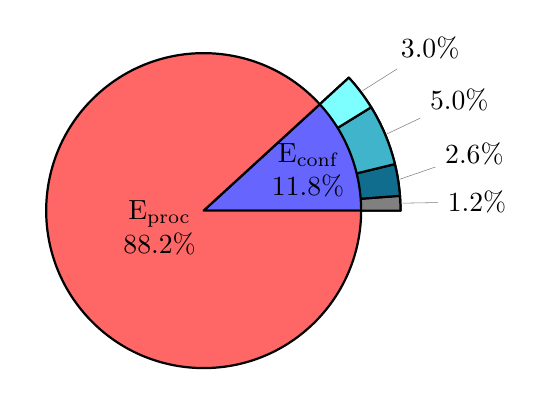
\begin{tikzpicture}
    \pie[
        radius=2.5,
        text=pin,
        hide number,
    ]{
        1.2/1.2\%,
        2.6/2.6\%,
        5.0/5.0\%,
        3.0/3.0\%
    }
    \pie[
        radius=2.5,
        hide number,
        color={gray, bluehue2, bluehue4, bluehue6},
        before number=\printonlylargeenough{2},
        after number=\ifprintnumber\%\fi
    ]{
        1.2/,
        2.6/,
        5.0/,
        3.0/
    }
    \pie[
        radius=2,
        text=inside,
        color={blue!60, red!60},
    ]{
        11.8/$\econf$,
        88.2/$\eproc$
    }
\end{tikzpicture}

    }
    \caption{Average energy consumption distribution of the models listed in \cref{tab:example_models_stats}}
    \label{fig:example_models_avg_conf_proc}
\end{figure}
    
% \section{Power analysis calculations}
The calculation for the total energy cost for configuring the \graicore{} and processing an input frame will be explained next.

\subsection{Configuration}
The configuration energy consists of the reading, transferring and writing of data from the external memory to the \graicore{}'s SRAMs. 

Let $C$ be the set of tuples holding the coordinates of every core:
\begin{equation}
    C = \{\,\left(x,y\right) \in \mathbb{N}^2 \mid 1 \leq x \leq 12 \wedge 0 \leq y \leq 11 \,\} 
\end{equation}

% \Cref{fig:model_data_heapmap} shows the amount of data from an arbitrary model that needs to be written to each of the 144 neuron cores.
\Cref{fig:model_data_heapmap} shows for a 80\% pruned version of ResNet-50\footnote{Internally named \texttt{resnet50\_pruned80\_star}} the amount of data that needs to be written to each of the 144 neuron cores.
We observe that the data is not uniformly distributed across the SRAMs.
Therefore, we require information how much data needs to be transferred to each SRAM.

\begin{figure}[hbtp]
    \centering
    \includegraphics[width=0.8\linewidth]{assets/model_data_heatmap.png}
    \caption{Amount of data to be written to each core for the ResNet-50 model (80\% pruned).}
    \label{fig:model_data_heapmap}
\end{figure}

Let $D$ be a matrix of $12 \times 13$ with $D_{i,j}$ denoting the amount of bytes to be written to core $\left( i,j \right)$.
$D$ has an additional column due to the x-coordinates not starting from index $0$.
Its left-most column is unused (i.e., $D_{0,0}, D_{0,1}, \cdots, D_{0,11}$).
This matrix can be constructed from the artifacts outputted by the compiler.

The number of phits to be transferred through the \confignoc{} influences the total energy costs.
In particular, the amount of phits to be transferred affects the number of hops to be taken in total and the amount of data to be written to the SRAMs.
Therefore, we need to determine how many phits needs to be transferred to each neuron core.
% The number of phits to be transferred influences the energy cost in the \confignoc{} hops and SRAM writes.
% A packet can contain up to 520 bytes\footnote{$65 \times \frac{64}{8}$} of payload data. 
A packet can contain up to 65 data phits, that is $65 \times \SI{64}{b} = \SI{520}{B}$ of payload data.
% If we transfe
Suppose we need to transfer $d$ bytes to a neuron core, we then require a total of $\left\lfloor \frac{d}{520} \right\rfloor$ packets with 65 data phits.
% If $d \bmod 520 > 0$, then there is an additional packet consisting of $\left\lceil \frac{\left( d \bmod 520 \right) \times 8}{64}\right\rceil$ data phits.
If $\left( d \bmod 520 \right) > 0$, then there is an additional packet for the remaining $\left( d \bmod 520 \right)$ bytes of data.
The remaining packet will consist of $\left\lceil \frac{d \bmod 520}{8}\right\rceil$ data phits.
Note that each packet also contains a single phit of 64 bits for the header information.


The total energy cost for configuring the \graicore{} can be estimated with the following equation:
\begin{equation}
    E_{\textrm{config}} = E_{\textrm{ext\_mem}} + E_{\textrm{noc}} + E_{\textrm{write}}
\end{equation}

With:
\begin{align*} 
E_{\textrm{ext\_mem}} &= 
        \sum_{c \in C}^{}{E_\textrm{read\_ext\_mem}(D_c) + E_{\textrm{send\_to\_noc}}(D_c)} \\
E_{\textrm{noc}} &=
    E_{\textrm{hop}} \times \sum_{c \in C}^{}{N_\textrm{hops}(c) \times p_{\textrm{total}}(D_c)} \\
E_{\textrm{write}} &=
    E_{\textrm{sram\_write\_64b}} \times \sum_{c \in C}^{}{p_{\textrm{data}}(D_c)}
\end{align*}

And:
\begin{align*} 
N_{\textrm{hops}}(x,y) &=
    \begin{cases} 
        x + y & \textrm{if } 0 \leq y \leq 5 \\
        x + y - 6 & \text{if } 6 \leq y \leq 11
    \end{cases}
\\
p_{\textrm{total}}(d) &=
    \left\lfloor \frac{d}{520} \right\rfloor \times (65 + 1) + \left\lceil \frac{d \bmod 520}{8} \right\rceil + 1 =
    \left\lceil \frac{d}{8} \right\rceil + \left\lfloor \frac{d}{520} \right\rfloor + 1 
\\
p_{\textrm{data}}(d) &=
    \left\lfloor \frac{d}{520} \right\rfloor \times 65 + \left\lceil \frac{d \bmod 520}{8} \right\rceil =
    \left\lceil \frac{d}{8} \right\rceil
\end{align*}

\begin{eqexpl}[15mm]
    \item{$p_{\textrm{total}}(D_c)$} total phits (includes headers) for transferring $D_c$ bytes
    \item{$p_{\textrm{data}}(D_c)$} total data phits (excludes headers) for transferring $D_c$ bytes
    \item{$N_{\textrm{hops}}(c)$} the amount of hops required to reach a neuron core at coordinate $c$, starting from the router closest to the injection point. It has two sub-functions due to the new \confignoc{}'s dual injector architecture
    \item{$E_{\textrm{read\_ext\_mem}}(D_c)$} energy for reading $D_c$ bytes from the external memory
    \item{$E_{\textrm{send\_to\_noc}}(D_c)$} energy for sending $D_c$ bytes from the external memory to the \confignoc{}
    \item{$E_{\textrm{hop}}$} energy for performing a single hop in the \confignoc{}
    \item{$E_{\textrm{sram\_write\_64b}}$} energy for writing back 64 bits to a neuron core's SRAM
\end{eqexpl}

\subsection{Processing}
The frame processing energy is the energy consumed when the \graicore{} processes a single frame with a configured model.
The energy for processing a single input frame is approximated as follows:
\begin{equation}
    E_{\textrm{frame}} = \textrm{avg\_util} \times \textrm{cores\_used} \times \textrm{processing\_latency} \times \SI{21}{mW}
\end{equation}

These parameters can all be extracted from \graipefruit{} simulation results.
% Suppose we have a large model that does not fit on the \graicore{} at once.
We will look at two strategies to partition the model to allow it to be executed on the \graicore{}.

Assume we have a model of that requires \SI{60}{MiB} to be written to the \graicore{}.
We are able to partition this model in two parts of \SI{30}{MiB} and four parts of \SI{15}{MiB}.
Furthermore, assume the latencies for processing and configuring as shown in \cref{tab:partitiong_strategies_example}.

\begin{table}[hbtp]
\centering
\begin{tabular}{@{}lll@{}}
\toprule
\textbf{Part} & \textbf{Processing (ms)} & \textbf{Configuration (ms)} \\ \midrule
\SI{30}{MiB}  & 4                        & 8                           \\
\SI{15}{MiB}  & 2                        & 4                          
\end{tabular}
\caption{TODO}
\label{tab:partitiong_strategies_example}
\end{table}

\section{Sequential configuration}
With the model partitioned in two parts of \SI{30}{MiB}, we can only fit one part on the \graicore{} at a time.
Because of this, we can only configure and process in a sequential manner.
The configure and process timeline is illustrated in \cref{fig:schedule_sequential_configuration}.
% In total, to fully process the model in two parts, it takes \SI{16}{ms}.
The inference latency of a single input frame is \SI{16}{ms}.
\Cref{fig:schedule_sequential_configuration_extended} shows a timeline when processing multiple input frames in sequence, we see that we can reach a stable input frame rate of \SI{41.7}{FPS} ($\frac{1}{\SI{24}{ms}}$).

\begin{figure}[hbtp]
    \centering
    \resizebox{0.6\linewidth}{!}{
        \begin{RTGrid}[
    width=10cm,
    nosymbols=1,
]{2}{26}
    \RowLabel{1}{Configure}
    \RowLabel{2}{Process}

    \TaskExecution[execlabel=$p_1$,color=lightgray]{1}{0}{8}
    \TaskExecution[execlabel=$p_2$,color=lightgray]{1}{12}{20}

    \TaskExecution[execlabel=$p_1$,color=lightgray]{2}{8}{12}
    \TaskExecution[execlabel=$p_2$,color=lightgray]{2}{20}{24}
\end{RTGrid}
    }
    \caption{Example timeline of sequential configuration and processing}
    \label{fig:schedule_sequential_configuration}
\end{figure}

\begin{figure}[hbtp]
    \centering
    \resizebox{1.0\linewidth}{!}{
        \begin{RTGrid}[
    width=20cm,
    nosymbols=1,
]{2}{52}
    \RowLabel{1}{Configure}
    \RowLabel{2}{Process}

    \TaskExecution[execlabel=$p_1$,color=lightred]{1}{0}{8}
    \TaskExecution[execlabel=$p_2$,color=lightred]{1}{12}{20}

    \TaskExecution[execlabel=$p_1$,color=lightred]{2}{8}{12}
    \TaskExecution[execlabel=$p_2$,color=lightred]{2}{20}{24}

    \TaskExecution[execlabel=$p_1$,color=lightcyan]{1}{24}{32}
    \TaskExecution[execlabel=$p_2$,color=lightcyan]{1}{36}{44}

    \TaskExecution[execlabel=$p_1$,color=lightcyan]{2}{32}{36}
    \TaskExecution[execlabel=$p_2$,color=lightcyan]{2}{44}{48}

    \TaskRespTime{2}{0}{8}
    \TaskRespTime{2}{24}{8}
    
    % \TaskArrival{2}{8}
    \TaskDeadline{2}{24}
    % \TaskArrival{2}{32}
    \TaskDeadline{2}{48}
\end{RTGrid}
    }
    \caption{
    Example timeline of sequential configuration and processing for two input frames.
    The shaded areas represent periods where we expect an input frame.
    The arrows pointing down represent the points of time where the associated input frame has been fully processed.
    }
    \label{fig:schedule_sequential_configuration_extended}
\end{figure}

\section{Parallel configuration}
With the model partitioned in four parts, two parts of \SI{15}{MiB} can fit on the \graicore{} at the same time.
This allows for a pipeline of configuration and processing.
For this approach to work, the neuron cores must be divided into two isolated segments/zones.
% With each zone able to contain a part.
Each of the zones will contain a single part.
With the introduction of the additional injection point, two model parts can be written to the local memories of the neuron cores in parallel.

\begin{figure}[hbtp]
    \centering
    \resizebox{0.65\linewidth}{!}{
        \begin{RTGrid}[
    width=10cm,
    nosymbols=1,
]{4}{26}
    \RowLabel{1}{Configure $Z_1$}
    \RowLabel{2}{Configure $Z_2$}
    \RowLabel{3}{Process $Z_1$}
    \RowLabel{4}{Process $Z_2$}

    \TaskExecution[execlabel=$p_1$,color=lightgray]{1}{0}{4}
    \TaskExecution[execlabel=$p_3$,color=lightgray]{1}{6}{10}

    \TaskExecution[execlabel=$p_2$,color=lightgray]{2}{0}{4}
    \TaskExecution[execlabel=$p_4$,color=lightgray]{2}{8}{12}

    \TaskExecution[execlabel=$p_1$,color=lightgray]{3}{4}{6}
    \TaskExecution[execlabel=$p_3$,color=lightgray]{3}{10}{12}

    \TaskExecution[execlabel=$p_2$,color=lightgray]{4}{6}{8}
    \TaskExecution[execlabel=$p_4$,color=lightgray]{4}{12}{14}
\end{RTGrid}
    }
    \caption{Example timeline of parallel configuration and processing}
    \label{fig:schedule_parallel_configuration}
\end{figure}

% This approach allows configuration of the two ``zones'' to be performed in parallel (see \cref{fig:schedule_parallel_configuration}).
% Also, processing and configuration can happen in parallel.
\Cref{fig:schedule_parallel_configuration} shows a timeline of a pipelined configuration and processing.
With this approach, the a constraint is that while the system is processing part $p_n$, the system should not reconfigure the zone where part $p_n$ resides at the same time.
$Z_1$ and $Z_2$ indicate one of the two independent zones.
Note that processing cannot be performed in parallel due to the input of the next part being dependent on the previous part's output.
% The following figure shows the timeline using ASAP scheduling for the tasks.
Observe that the configuration of $p_2$ can start \SI{2}{ms} later without affecting the total inference latency.
The total inference latency of this approach is \SI{10}{ms}.
This is a speedup of $1.6\times$ compared to the sequential configuration approach.
% with \SI{100}{FPS} ($\frac{1}{\SI{10}{ms}}$) as the highest manageable input frame rate.
% However, this does not allow for an input frame rate of \SI{100}{FPS} ($\frac{1}{\SI{10}{ms}}$).

\Cref{fig:schedule_parallel_configuration_extended} shows a possible timeline for three consecutive input frames at the highest manageable frame rate.
An arrow pointing up shows the arrival of an input frame.
It is apparent that the highest manageable frame rate is \SI{83.3}{FPS} ($\frac{1}{\SI{12}{ms}}$).

\begin{figure}[hbtp]
    \centering
    \resizebox{0.8\linewidth}{!}{
        \begin{RTGrid}[
    width=15cm,
    nosymbols=1,
]{4}{38}
    \RowLabel{1}{Configure $Z_1$}
    \RowLabel{2}{Configure $Z_2$}
    \RowLabel{3}{Process $Z_1$}
    \RowLabel{4}{Process $Z_2$}

    \TaskExecution[execlabel=$p_1$, color=lightred]{1}{0}{4}
    \TaskExecution[execlabel=$p_3$, color=lightred]{1}{6}{10}

    \TaskExecution[execlabel=$p_2$, color=lightred]{2}{0}{4}
    \TaskExecution[execlabel=$p_4$, color=lightred]{2}{8}{12}

    \TaskExecution[execlabel=$p_1$, color=lightred]{3}{4}{6}
    \TaskExecution[execlabel=$p_3$, color=lightred]{3}{10}{12}

    \TaskExecution[execlabel=$p_2$, color=lightred]{4}{6}{8}
    \TaskExecution[execlabel=$p_4$, color=lightred]{4}{12}{14}
    %%%
    \TaskExecution[execlabel=$p_1$, color=lightcyan]{1}{12}{16}
    \TaskExecution[execlabel=$p_2$, color=lightcyan]{2}{14}{18}

    \TaskExecution[execlabel=$p_1$, color=lightcyan]{3}{16}{18}
    \TaskExecution[execlabel=$p_2$, color=lightcyan]{4}{18}{20}

    \TaskExecution[execlabel=$p_3$, color=lightcyan]{1}{18}{22}
    \TaskExecution[execlabel=$p_4$, color=lightcyan]{2}{20}{24}

    \TaskExecution[execlabel=$p_3$, color=lightcyan]{3}{22}{24}
    \TaskExecution[execlabel=$p_4$, color=lightcyan]{4}{24}{26}
    %%%
    \TaskExecution[execlabel=$p_1$, color=lightgreen]{1}{24}{28}
    \TaskExecution[execlabel=$p_2$, color=lightgreen]{2}{26}{30}

    \TaskExecution[execlabel=$p_1$, color=lightgreen]{3}{28}{30}
    \TaskExecution[execlabel=$p_2$, color=lightgreen]{4}{30}{32}

    \TaskExecution[execlabel=$p_3$, color=lightgreen]{1}{30}{34}
    \TaskExecution[execlabel=$p_4$, color=lightgreen]{2}{32}{36}

    \TaskExecution[execlabel=$p_3$, color=lightgreen]{3}{34}{36}
    \TaskExecution[execlabel=$p_4$, color=lightgreen]{4}{36}{38}
    %%%
    % \TaskArrival{3}{4}
    % \TaskArrival{3}{16}
    % \TaskArrival{3}{28}
    
    \TaskRespTime{3}{0}{4}
    \TaskRespTime{3}{14}{2}
    \TaskRespTime{3}{26}{2}
    
    \TaskDeadline{4}{14}
    \TaskDeadline{4}{26}
    \TaskDeadline{4}{38}
\end{RTGrid}

    }
    \caption{
    Example timeline of parallel configuration and processing for three input frames.
    The shaded areas represent periods where we expect an input frame.
    The arrows pointing down represent the points of time where the associated input frame has been fully processed.
    }
    \label{fig:schedule_parallel_configuration_extended}
\end{figure}



\newpage
\printbibliography[heading=bibintoc]

\end{document}
